\documentclass[times, utf8, zavrsni]{fer}
\usepackage{booktabs}
\usepackage{makecell}
\usepackage{longtable}
\usepackage{float}
\begin{document}
	
	
	\title{Rješavanje problema smještanja i povezivanja kod sklopa FPGA}
	
	% Dodavanje zahvale ili prazne stranice. Ako ne želite dodati zahvalu, naredbu ostavite radi prazne stranice.
	\zahvala{}
	
	\tableofcontents
	
	\chapter{Uvod}
	
	\section{Evolucijsko računarstvo}
	
	Evolucijsko računarstvo (eng. \emph{Evolutionary computing}) je područje računarske znanosti koje se bavi problemom optimizacije složenih funkcija, a nastali su proučavanjem procesa u prirodi. Preciznije bismo evolucijsko računarstvo mogli svrstati u područje umjetne inteligencije (eng. \emph{artificial intelligence}) i mekog računarstva (eng. \emph{soft computing}).\\Roditeljski koncept na kojem se temelji jest pojam metaheuristika (eng. \emph{metaheuristics}), a to je pak vrlo općenita heuristika čija je zadaća pomoći heuristici specifičnoj problemu, pri usmjeravanju prema prostoru u kojem se nalaze potencijalno dobra rješenja konkretnog problema. Evolucijsko računarstvo možemo podijeliti na evolucijske algoritme u koje spadaju genetski algoritmi, genetsko programiranje, evolucijske strategije, evolucijsko programiranje, kategoriju koju predstavljaju algoritmi rojeva, a u koje ubrajamo mravlje algoritme, algoritme roja čestica, algoritme pčela i dr. te zadnju skupinu algoritama koju čine umjetni imunološki algoritmi, algoritam diferencijske evolucije te algoritam harmonijske pretrage.\\
	Evolucijski algoritmi se koriste kako bi dobro aproksimirali rješenja problema koji se ne mogu jednostavno rješiti primjenom nekih drugih koncepata, npr. tehnikom grube sile. Čest problem koji se rješava evolucijskim računarstvom je problem raspoređivanja, a upravo se ovaj rad bavi razmještanjem i konfiguriranjem logičkih blokova, ulaza i izlaza kod FPGA sklopa (eng. \emph{field- programmable gate array}). Za raspoređivanje koristim genetski algoritam koji je jedan od najčešće korištenih algoritama iz područja evolucijskog računarstva u problemima raspoređivanja.\\
	Najprije ću opisati princip rada FPGA sklopa i samih genetskih algoritama. Nakon toga prezentirati ću implementaciju sustava koji je sposoban rješiti navedeni problem, navesti njegove prednosti, nedostatke i ograničenja u uporabi. Rezultati su prezentirani kroz tablice, grafove i slike generiranih rješenja. 
	
	\section{FPGA sklop}
	
	\subsection{Arhitektura FPGA sklopa}
	
	FPGA je digitalni sklop koji se koristi za realiziranje funkcija specificiranih od strane programera uporabom sklopovski specifičnih jezika za programiranje. Primjer jednog takvog jezika je VHDL.\\ Najosnovnija arhitektura FPGA sklopa podrazumijeva ulazno-izlazne spojeve (eng. \emph{pin}) na koje se dovode ulazi željenih funkcija i odvode izlazi. Središnji dio sklopa čine LUT tablice (eng. \emph{lookup table}). One imaju $2^n$ zapisa, a svaki je zapis zadužen za pojedinu kombinaciju ulaznih varijabli. LUT tablice su dio CLB-ova (eng. \emph{configurable logic blocks}) na koje se dovode žice. Napomenimo kako su LUT tablice samo jedan od mogućih načina izvedbe, druge često korištene tehnike podrazumijevaju korištenje multipleksera i jednostavnih flip-flop bistabila. Žice najčešće ne dolaze samostalno već u snopovima i one su zadužene za provođenje signala dobivenog od ulaznih varijabla. Prospojne kutije (eng. \emph{switch box}) spajaju žice koje se nalaze u susjednim snopovima. Ovisno o poziciji prospojne kutije moguće jest da jedna prospojna kutija spaja dva, tri ili četiri susjedna snopa žica.\\ Primijetimo na temelju slike 1.1 kako u najopćenitijem slučaju dvije žice možemo spojiti na \emph{n} načina pa ne postoji nužno samo jedna ispravna konfiguracija konkretne prospojne kutije za ostvarenje željenog spoja.
	
	\begin{figure}[H]
		\centering
		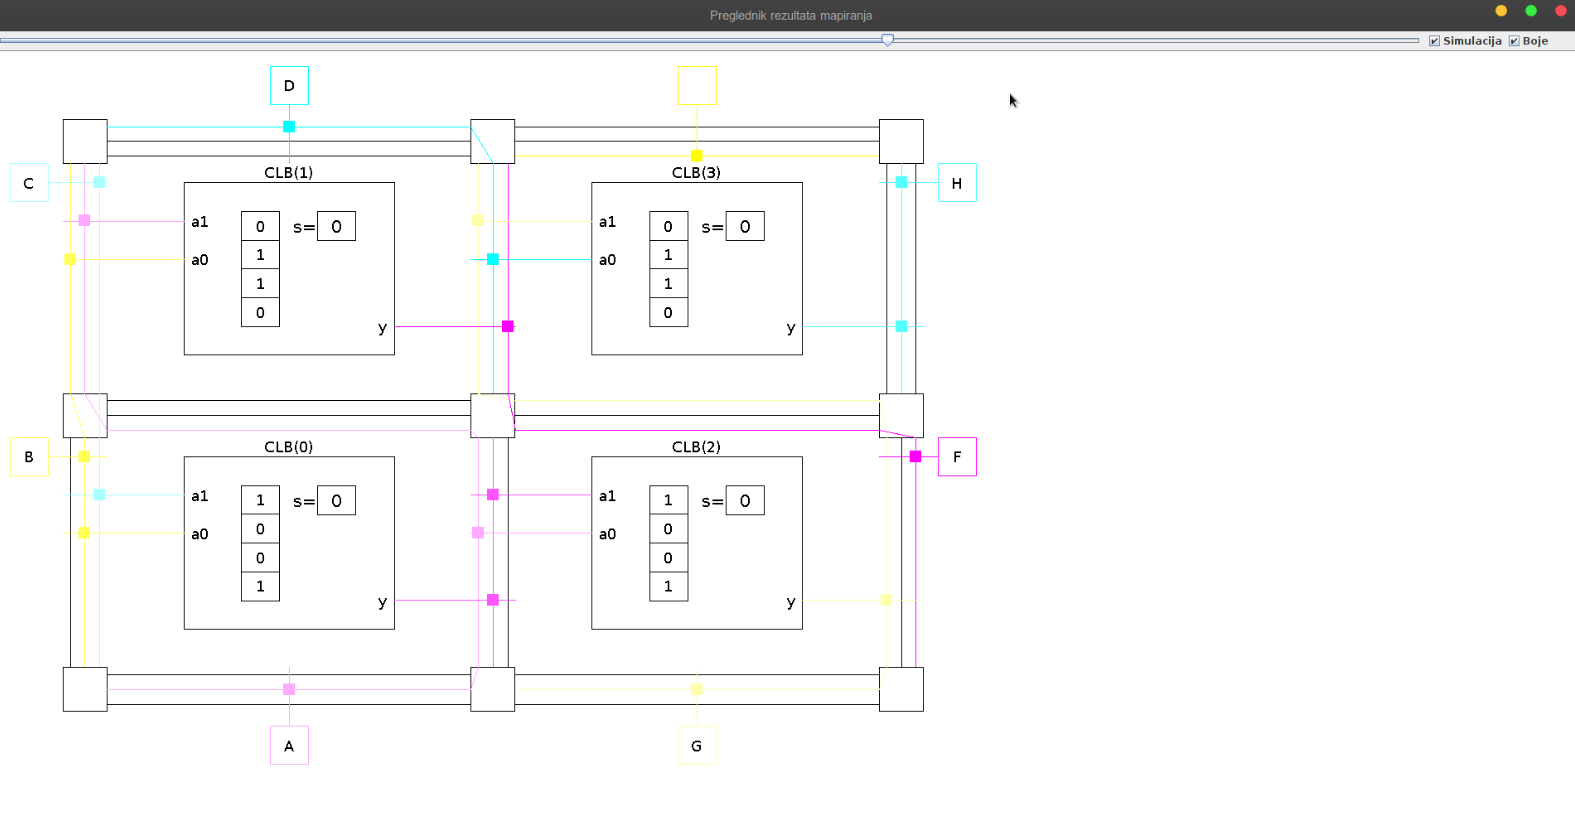
\includegraphics[width=20cm]{slike/arhFPGA.png}
		\caption{Arhitektura FPGA sklopa s četiri dvoulazna CLB sklopa i tri žice u snopu. Fizički pogled na sklop.}
		\label{fig:arh-fpga}
	\end{figure}
	
	\subsection{Programski model FPGA sklopa}
	
	Implementacija cijelog sustava pisana je u programskom jeziku Java, a korištene su tehnologije Java 15 SDK za programiranje, Maven za upravljanje projektom, Github za verzioniziranje sustava i Java Swing za stvaranje grafičkih korisničkih sučelja (eng. \emph{GUI}).\\ Model FPGA sklopa možemo definirati na dva načina: prvi ćemo zvati fizički model jer promatramo FPGA sklop kao stvarni fizički sustav i za njega pamtimo ono što imamo na raspologanju. Kod njega je specificirano koliko CLB-ova imamo na raspologanju, broj ulaza koji se dovode na svaki CLB, broj žica koje se nalaze u jednom snopu, broj UI spojeva po svakom CLB-u, konfiguracija svih prospojnih kutija te signali koji se nalaze na pojedinoj žici.\\Druga mogućnost je opisivanje FPGA sklopa kao objekt koji želimo ostvariti i taj ćemo način opisivanja zvati logički model. Njega zadajemo pomoću tekstualne datoteke u kojoj su navedeni potrebni parametri.\\Nakon opisa fizičkog i logičkog modela FPGA sklopa sada nam je lakše uvidjeti što je programski cilj ovog rada: uporabom genetskog algoritma logički model mapirati u fizički sustav. Možemo izvesti analogiju sa stvarnim životom u kojem je fizički model kutija u koju pokušavamo ubaciti specifični objekt na način da zadovoljava osnovne zahtjeve kutije.
	
	
	\begin{figure}[H]
		\centering
		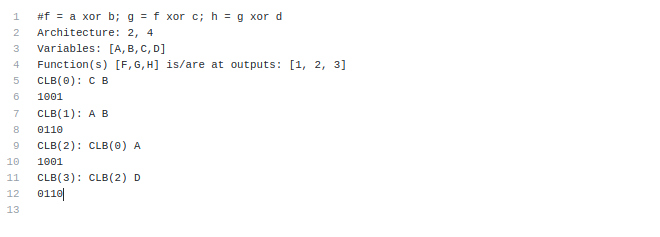
\includegraphics[width=15cm]{slike/logicalModelTxt.png}
		\caption{Primjer zadavanja logičkog modela FPGA sklopa. Za svaki CLB piše koje točno varijable dovodimo, programiranje LUT tablice i koje funkcije želimo ostvariti na kojem izlazu. }
		\label{fig:fpga-logical-model}
	\end{figure}
	
	
	\chapter{Genetski algoritmi}
	
	\section{Princip rada}
	
	Genetski se algoritam zasniva na populaciji rješenja i najčešće se slučajnim procesima nasumično stvaraju početne jedinke. U složenijim problemima moguće je, prije pokretanja evolucijskog računanja, na temelju neke jednostavne heuristike izgraditi startnu populaciju. Takav pristup u većini slučajeva ubrzava konvergiranje algoritma. Populacija se s vremenom mijenja, a za to je zadužen proces selekcije, ali više o njemu u poglavlju o selekciji. Za sada ćemo samo spomenuti da selekcija ne mijenja nužno loše jedinke. Dapače, moguće je da proces algoritam iz nasumično odabranih roditeljskih jedinki stvori nekvalitetnu jedinku dijete i zamijeni ju s najboljom jedinkom iz roditeljske populacije. Kroz rad ćemo se upoznati s elitističkim pristupom koji rješava taj problem. \\
	
	\begin{figure}[!htb]
		\centering
		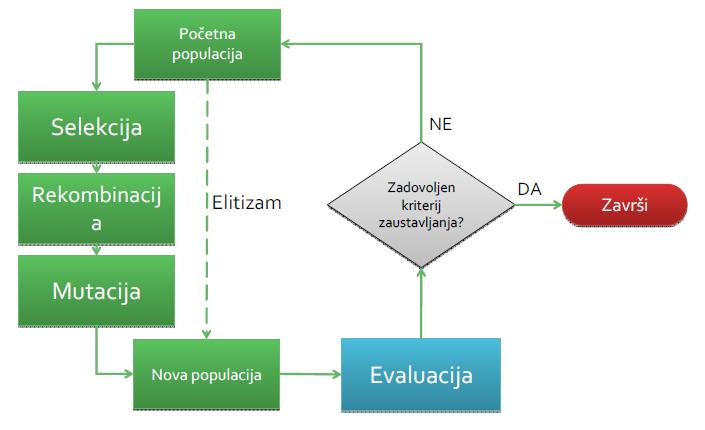
\includegraphics[width=15cm]{slike/genetskiGeneral.jpg}
		\caption{Koraci u radu genetskog algoritma. }
		\label{fig:genetic-general}
	\end{figure}
	
	Genetski se algoritam može definirati kao heuristika pretraživanja koja inspiraciju temelji na Charles Darwinovoj teoriji evolucije. Ta se teorija temelji na 5 osnovnih pretpostavki: 
	\begin{enumerate}
		\item plodnost vrsta - potomaka ima uvijek više, no što je potrebno,
		\item veličina populacije je približno stalna,
		\item količina hrane je ograničena,
		\item kod vrsta koje se seksualno razmnožavaju, nema identičnih jedinki već postoje varijacije te
		\item najveći dio varijacija prenosi se nasljeđem. [\citep{PIOA}]
		
	\end{enumerate}
	
	\begin{figure}[!htb]
		\centering
		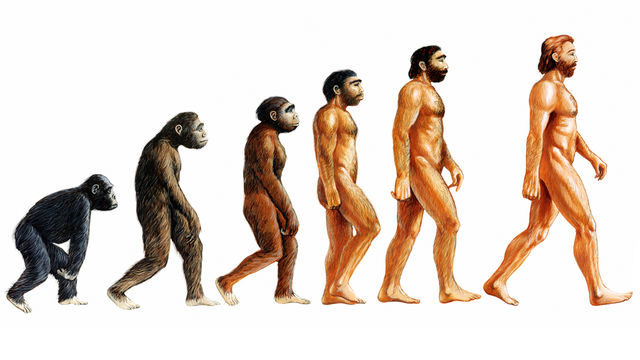
\includegraphics[width=15cm]{slike/darwin.jpg}
		\caption{Darwinova teorija evolucije. Iz generacije u generaciju vrijednost funkcije dobrote prosječno raste.}
		\label{fig:darwin}
	\end{figure}
	
	Algoritam preslikava proces prirodne evolucije gdje su neke jedinke primjenom evolucijskog operatora selekcije izabrane kao roditelji koji će sudjelovati u procesu križanja kako bi stvorili genetski materijal jedinke djeteta. Postoji nebrojeno puno inačica genetskog algoritma, ali osnovna ideja je sljedeća: algoritam radi s populacijom jedinki pri čemu je svaka jedinka potencijalno rješenje problema i nju nazivamo kromosomom. Za svaku jedinku računamo  funkciju dobrote (eng. \emph{fitness}), a ona može biti izvedena kao funkcija nagrade, funkcija kazne ili pak hibrid. Cilj je da funkcija dobrote vjerno oslikava kvalitetu pojedine jedinke pa je, ovisno o vrsti problema, cilj minimizirati ili maksimizirati funkciju dobrote. Korištenjem evolucijskog operatora selekcije odabiru se kromosomi koji će sudjelovati u rekombinaciji gena s ciljem stvaranja bolje jedinke. Taj postupak nazivamo križanje. Mutacijom mijenjamo pojedine gene kromosoma kako bismo dodatno utjecali na prostor pretraživanja stanja. Operatorom zamjene mijenjamo jedinku iz roditeljske populacije s novom jedinkom kako bismo očuvali veličinu populacije. 
	
	\section{Traženje rješenja}
	
	Genetski algoritam služi za rješavanje težih optimizacijskih problema, za koje ne postoji egzaktna matematička metoda rješavanja ili su NP teški problemi pa se za veći broj nepoznanica ne mogu riješiti u razumnom vremenu [\citep{NENR}]. To radi na način da pretražuje prostor stanja pa formalno možemo predstaviti genetski algoritam kao složenu funkciju $g : J^N$$=>$$J^N$ koja uz pomoć genetskih operatora preslikava roditeljsku populaciju u novu populaciju. 
	
	\begin{figure}[!htb]
		\centering
		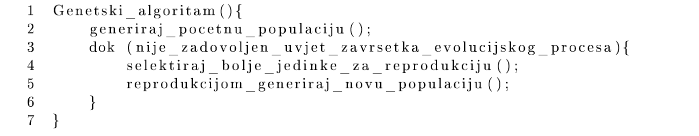
\includegraphics[width=15cm]{slike/nenrGenAlg.png}
		\caption{Ciklički proces rada genetskog algoritma. }
		\label{fig:nenr-alg}
	\end{figure}
	
	
	Sada smo sposobni definirati proces stvaranja genetskog algoritma. Prvi je korak odrediti prikaz jedinke. Tu možemo genetski algoritam podijeliti na one koji rade s bitovima i na one koji rade s nekakvom drugom strukturom podataka. U većini je slučajeva najpogodnije raditi sa strukturom polje (eng. \emph{array}) jer algoritam radi sa fiksnom veličinom populacije pa operacije dohvaćanja, postavljanja i zamjene možemo raditi u O(1) vremenskoj složenosti (eng. \emph{big O notation}). Nakon toga slijedi fino podešavanje parametara genetskog algoritma kako bismo dobili što je moguće bolje rješenje. Nerijetko se u praksi parametri najprije odrede na temelju nekog jednostavnog problema, nakon čega se prelazi na glavni slučaj. Ovisno o izvedbi, dijelovi algoritma se paraleliziraju kako bi se maksimalno ubrzalo izvođenje. Spomenimo za kraj ovog dijela kako genetski algoritam nije deterministički algoritam koji uvijek pronađe najbolje rješenje, već postupak koji u zadanom vremenu pronalazi najkvalitetnije moguće. 
	
	\section{Evolucijski operatori}
	
	\subsection{Selekcija}
	\label{selekcija}
	
	Selekcija je evolucijski operator čiji je zadatak osigurati da bolje jedinke češće sudjeluju u produkciji novih rješenja kako bismo usmjerenim pretraživanjem došli u prostor koji nam može ponuditi optimalno rješenje. Takav mehanizam možemo opisivati kroz više parametara, a prvi od njih je vrijeme preuzimanja (eng. \emph{takeover time}). To je vrijeme potrebno operatoru selekcije da generira populaciju u kojoj se nalaze samo najbolja rješenje [\citet{GoldAndDeb}]. Radi se o tome da kada bi novu populaciju stvarali samo operatorom selekcije koji favorizira bolje jedinke, tada je logično očekivati da će u svakoj novoj generaciji biti sve više i više kopija najboljeg rješenja. Vrijeme preuzimanja se najčešće mjeri u generacijama, a za k-turnirsku selekciju aproksimativan izraz je odredio \citet{EvAlgsinTheoryAndPractise} 
	
	\begin{equation}
		\rho=\frac{1}{\ln{n}} (\ln{k} + \ln{(\ln{k})})) 
	\end{equation}
	
	gdje je n veličina populacije a k broj jedinki koje ulaze u turnir. Mehanizam selekcije promatra se i kroz selekcijski intenzitet koji se računa kao povećanje srednje dobrote populacije prije i nakon primjene operatora selekcije, podijeljeno sa standardnom devijacijom populacije: [\cite{Back1995, MillerAndGoldberg, MuhlenbeinAndVoosen, Thierens}]
	
	\begin{equation}
		\label{izraz}
		I=\frac{\bar{f_s} - \bar{f}}{\sigma}
	\end{equation}
	
	gdje je $\bar{f}$ prosječna dobrota rješenja u roditeljskoj populaciji, $\bar{f_s}$ prosječna dobrota rješenja u novoj populaciji, a $\sigma$ standardna devijacija dobrote rješenja u roditeljskoj populaciji. Iz izraza 2.2 vidimo kako je selekcijski intenzitet obrnuto proporcionalan standardnoj devijaciji, ali dokazana je i puno jača tvrdnja prema kojoj je selekcijski intenzitet obrnuto proporcionalan brzini konvergencije. 
	
	\begin{equation}
		\sigma=\frac{1}{n}\sum_{1}^{n}(f_i - \bar{f})^2
	\end{equation}
	
	\begin{figure}[!htb]
		\centering
		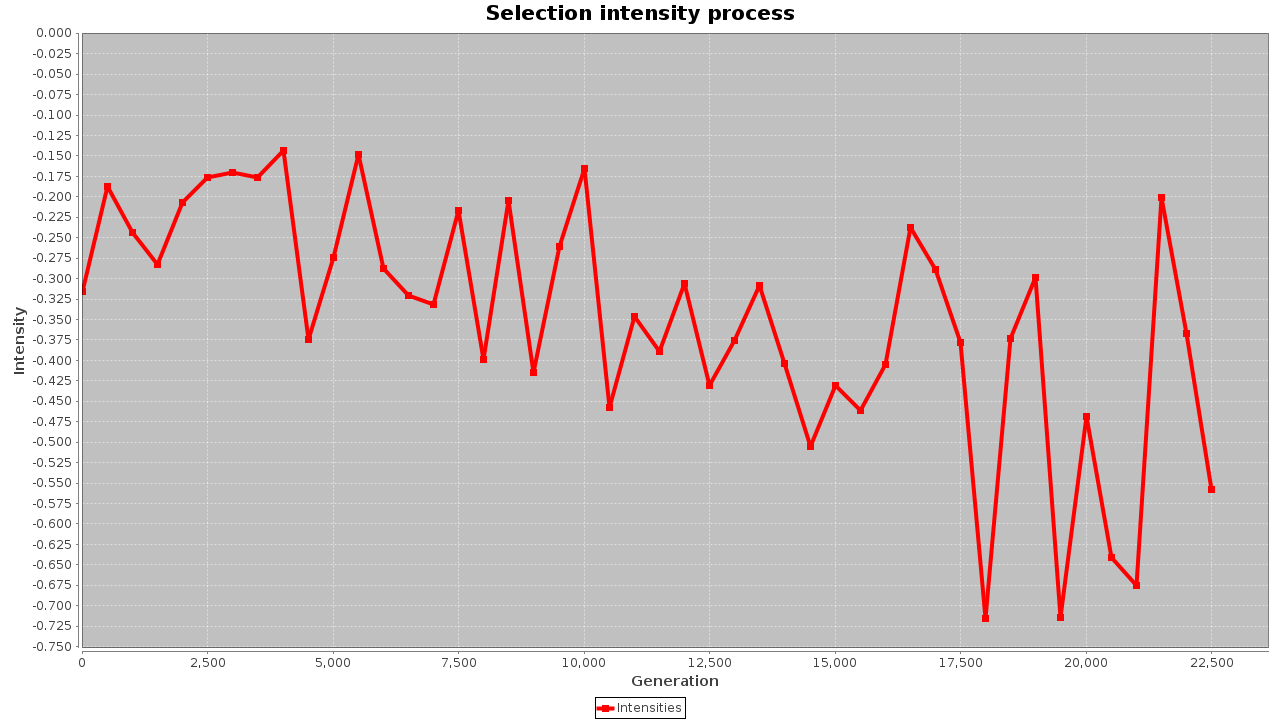
\includegraphics[width=15cm]{slike/intensity.png}
		\caption{Selekcijski intenzitet se smanjuje kako se smanjuje standardno odstupanje i povećava srednja vrijednost populacije. }
		\label{fig:k-tour-select}
	\end{figure}
	
	Drugi parametri koji se koriste u okviru selekcije nisu toliko česti pa ih preskačem. 
	
	Postoji velik broj selekcija, a u ovom radu ću se radu dotaknuti dvije najpoznatije, a to su k-turnirska selekcija i proporcionalna selekcija (eng. \emph{roulette-wheel selection}).
	
	\subsubsection{K-turnirska selekcija}
	K-turnirska selekcija spada u turnirske selekcije, a neki od ostalih predstavnika te grupe su binarna turnirska selekcija i Boltzmannova turnirska selekcija.
	Radi se o postupku u kojem se nasumičnim odabirom izabere k kromosoma i vrati najbolji od njih. Kod odabira roditelja najčešće se zabrajanjuje situacija u kojoj su oni jednaki. Selekcijski intenzitet kod turnirske selekcije je određen izrazom 
	
	\begin{equation}
		\sqrt{\sqrt{2} \ln{k}}
	\end{equation}
	
	gdje je k broj jedinki koji ulazi u turnir [\citep{Back1995}]. 
	
	\begin{figure}[!htb]
		\centering
		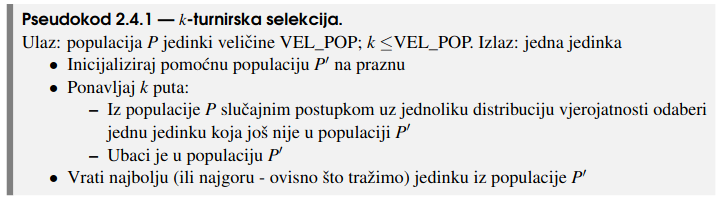
\includegraphics[width=15cm]{slike/kTourSelect.png}
		\caption{Pseudokod k-turnirske selekcije}
		\label{fig:k-tour-select}
	\end{figure}
	
	
	\subsubsection{Proporcionalna selekcija}
	\label{proportional-sel}
	Proporcionalna selekcija je najpoznatiji predstavnik grupe mehanizama selekcija koje svoj odabir temelje isključivo na dobroti jedinka. Kod ovog se postupka svakoj jedinki pridruži vjerojatnost odabira koja je proporcionalna njezinoj dobroti:
	
	\begin{equation}
		p_i=\frac{f_i}{\sum_{1}^{n}f_j}
	\end{equation}
	
	Ovakav mehanizam podrazumijeva da su dobrote svih jedinki nenegativne pa ih je nužno translatirati u prostor $R^+$. Translaciju je dobro napraviti i zbog poznatog problema skale. Naime, ako su dobrote približno jednaki veliki brojevi, onda su i vjerojatnosti odabira svake gotovo iste. Pretpostavimo da populacija ima 5 članova i da su njihove dobrote redom: 10000001, 10000002, 10000003, 10000004 i 10000005. Zadnja jedinka ima najveću vrijednost dobrote pa nju želimo sa što većom vjerojatnošću odabrati. Međutim, uz ovakve vrijednosti, vjerojatnosti njihovog odabira su identične do na 6. decimalu i iznose približno $\approx20\%$.  Translacijom za minimalnu vrijednost, u ovom slučaju 10000001, vrijednosti dobrota postaju 0, 1, 2, 3 i 4 pa je primjerice vjerojatnost odabira najbolje jedinke sada jednaka 40\%. \\
	Selekcijski intenzitet proporcionalne selekcije možemo izračunati izrazom:
	
	\begin{equation}
		I=\frac{\sigma}{\bar{f}}
	\end{equation}
	
	gdje se obje varijable odnose na trenutačnu populaciju s kojom radimo.
	
	\begin{figure}[!htb]
		\centering
		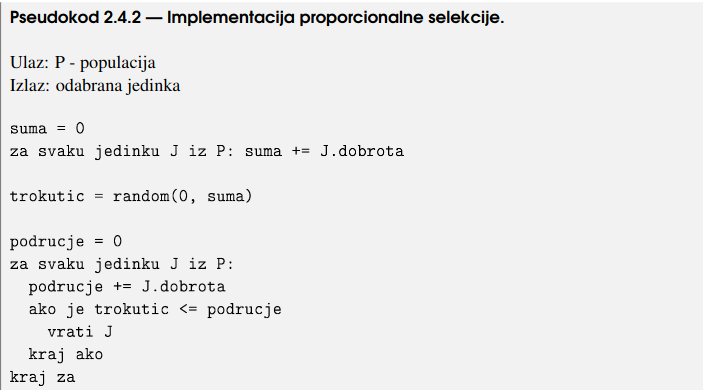
\includegraphics[width=15cm]{slike/proportionalSel.png}
		\caption{Pseudokod proporcionalne selekcije}
		\label{fig:proportional-selection}
	\end{figure}
	
	
	\subsection{Reprodukcija}
	
	\subsubsection{Križanje}
	
	Križanje je evolucijski operator koji stvara djecu. Izvedeno je iznimno puno načina križanja, ali svi imaju isti cilj: kombinirati gene roditelja kako bi se stvorilo što je moguće bolje dijete. \\Ako se vratimo na inicijalnu pretpostavku kako genetski algoritam pretražuje prostor rješenja onda je križanje fina pretraga u okolini jedinka roditelja. Takav način rada ima svoju prednost zbog toga jer na jako precizan način prolazi po jednom dijelu prostora rješenja, ali s druge strane moguće je da zbog toga izgubimo optimalnost. Uzmimo za primjer optimizacijski problem pronalaska maksimuma funkcije na nekom intervalu gdje se za operator križanja koristi aritmetička sredina. Ako selekcija u početku izbaci jedinku koja ima veliku vrijednost funkcije na nekom intervalu, ali ne na cijelom (lokalni optimum) tada će takvo križanje u tom smanjenom intervalu najvjerojatnije stvarno naći maksimum, ali to neće biti globalni optimum. \\Osim križanja aritmetičkom sredinom često se koristi križanje s jednom točkom prekida, križanje s više točka prekida i uniformno križanje. Kod križanja s jednom točkom prekida nasumičnim se odabirom odredi jedna točka do koje se u dijete ubacuju svi geni iz prvog roditelja, a od točke naprijed svi geni drugog roditelja. Uniformnim križanjem za svaki gen biramo roditelja te je takvo križanje neprikladno ukoliko nam je važna sekvenca gena, a ne samo jedan gen. Križanje s više točka prekida je analogno križanju s jednom točkom prekida samo što se geni prekidaju na više mjesta.
	
	\begin{figure}[H]
		\centering
		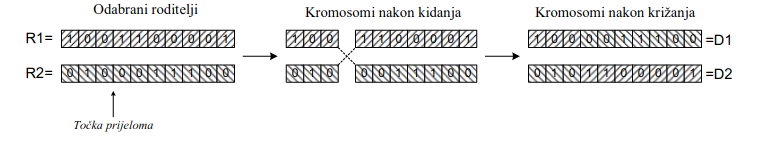
\includegraphics[width=12cm]{slike/crossOnePoint.png}
		\caption{Križanje s jednom točkom prijeloma}
		\label{fig:one-cross}
	\end{figure}
	
	\begin{figure}[H]
		\centering
		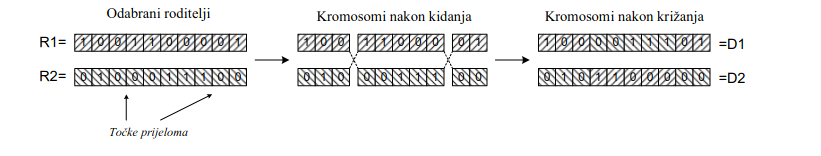
\includegraphics[width=12cm]{slike/crossTPoint.png}
		\caption{Križanje s više točka prijeloma}
		\label{fig:t-crosses}
	\end{figure}
	
	\subsubsection{Mutacija}
	
	Mutacija ima upravo suprotnu ulogu od križanja. Ona radi grubu pretragu prostora pretraživanja na način da promijeni određene gene i time izbaci jedinku iz potencijalno lokalnog optimuma i vrati je u širi prostor u kojem je moguće pronaći globalni. Upravo iz tog razloga mutacija povećava volumen populacije, a križanje smanjuje. 
	
	\paragraph{Mutacija zamjenom (eng. \emph{Swap mutation})}
	\label{SwapMutation}
	Kod ove vrste mutacije odaberemo dvije pozicije i geni se na tim pozicijama jednostavno zamjene.
	
	\paragraph{Mutacija premještanjem (eng. \emph{Cut mutation})}
	Slučajnim odabirom izaberemo dvije pozicije te sekvencu gena između njih stavimo iza treće nasumično odabrane pozicije. Geni koji su bili iza treće nasumično odabrane pozicije stavljamo na prvu slobodnu poziciju iza.
	
	\begin{figure}[!htb]
		\centering
		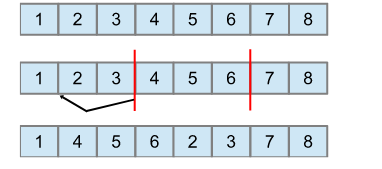
\includegraphics[width=8cm]{slike/cutMutation.png}
		\caption{Mutacija premještanjem}
		\label{fig:cut-mutation}
	\end{figure}
	
	\paragraph{Mutacija umetanjem (eng. \emph{Insertion mutation})}
	
	Slučajno se odabere jedna pozicija i iz te pozicije se uzme jedan gen koji se stavlja iza druge nasumično odabrane pozicije. 
	
	
	\begin{figure}[!htb]
		\centering
		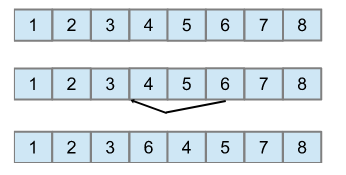
\includegraphics[width=8cm]{slike/ISM.png}
		\caption{Mutacija umetanjem}
		\label{fig:insertion-mutation}
	\end{figure}
	
	\paragraph{Jednostavna mutacija inverzijom (eng. \emph{Simple inversion mutation})}[\citep{Holland}]
	Nad kromosomom se odaberu dvije slučajne pozicije te se tako selektirani podniz prepiše obrnutim redoslijedom.
	
	
	\begin{figure}[!htb]
		\centering
		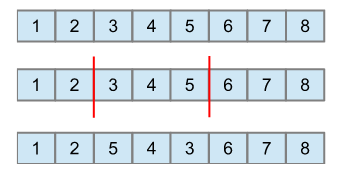
\includegraphics[width=8cm]{slike/SIM.png}
		\caption{Jednostavna mutacija inverzijom}
		\label{fig:inversion-mutation}
	\end{figure}
	
	\paragraph{Vjerojatnosna mutacija}
	
	Ovakva mutacija zahtijeva postojanje parametra koji određuje s kojom vjerojatnošću mijenjamo svaki gen. Taj parametar zvati ćemo \emph{$\alpha$}. Zatim za svaki gen u kromosomu računamo slučajnu vrijednost i ako je manja od parametra \emph{$\alpha$}, gen mutiramo. 
	
	\subsection{Parametri genetskog algoritma}
	
	U svakom genetskom algoritmu vrlo je važno pronaći dobar omjer između svih parametara koji se koriste, a pri tome se misli na:
	\begin{enumerate}
		\item veličinu populacije
		\item broj generacija
		\item način selekcije
		\item način mutiranja
		\item način križanja
	\end{enumerate}
	
	Također, važno je reći da ne postoje točne vrijednosti parametara, nego se do njih dolazi eksperimentiranjem i iskustvom. Posebice su nam bitni mutacija i križanje s kojima pretražujemo prostor rješenja. Ako je kontrakcijsko djelovanje mutacije prejako, ono će konzistentno uništavati sve pozitivno što je postupak pretraživanja do tada pronašao i pretragu će svesti na slučajnu [\citep{UI}]. Treba težiti tome da su mutacija i križanje u balansu kako bismo osigurali napredak u pretraživanju. 
	
	
	\begin{figure}[!htb]
		\centering
		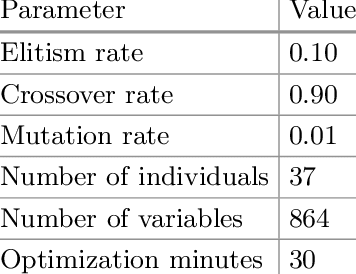
\includegraphics[width=6cm]{slike/genAlgParams.png}
		\caption{Primjer parametara genetskog algoritma}
		\label{fig:gen-params}
		
	\end{figure}
	
	
	\subsection{Eliminacijski genetski algoritam}
	
	Eliminacijski genetski algoritam u svakoj generaciji stvara samo jedno novo dijete i ubacuje ga na mjesto neke od roditeljske jedinke, najčešće je to najlošija jedinka. Najjednostavnija verzija tog algoritma nasumično odabire tri jedinke, križa bolje dvije i dijete stavlja na mjesto treće ako je bolje od nje.
	
	\begin{figure}[!htb]
		\centering
		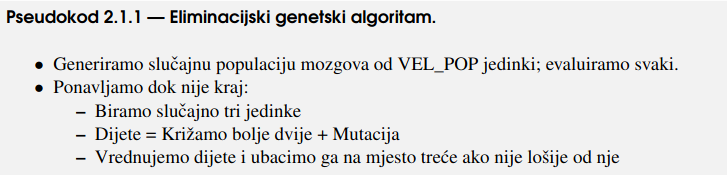
\includegraphics[width=15cm]{slike/elimGenAlg.png}
		\caption{Pseudokod eliminacijskog genetskog algoritma}
		\label{fig:elim-gen-alg}
	\end{figure}
	
	\subsection{Generacijski genetski algoritam}
	
	Generacijski genetski algoritmi u svakoj generaciji stvaraju potpuno novu populaciju te roditeljsku zamjenjuju populacijom djece. 
	
	
	\begin{figure}[htb]
		\centering
		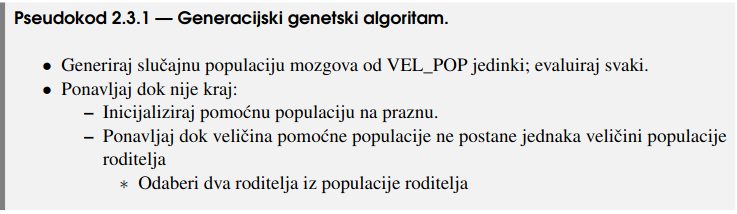
\includegraphics[width=15cm]{slike/genGenAlg.png}
		\caption{Pseudokod generacijskog genetskog algoritma}
		\label{fig:gen-gen-alg}
	\end{figure}
	
	\subsection{Elitizam}
	\label{elitizam}
	
	Elitizam je svojstvo algoritma da ne može izgubiti najbolje pronađeno rješenje [\citep{UI}]. Kod eliminacijske verzije ono je najčešće očuvano dok se kod generacijskog npr. to može jednostavno postići umetanjem jedinke na početak nove populacije.
	
	
	\chapter{Implementacija sustava}
	
	\section{Opis modela}
	
	Programski je dio završnog rada obuhvaćao izradu sustava koji je sposoban logički model mapirati u fizički model FPGA sklopa. Taj se sustav ne koristi sam za sebe već leži između dijela koji radi dekompoziciju Booleovih funkcija koje želimo ostvariti i dijela koji je zadužen za prikaz i simulaciju rada FPGA sklopa. Oba dijela su izrađena od strane izv. prof. dr. sc Marka Čupića. 
	
	\begin{figure}[!htb]
		\centering
		
\includegraphics[width=15cm]{slike/arhitekturaSustava.png}
		\caption{Arhitektura cijelog sustava koji se koristi}
		\label{fig:arh-sustav}
	\end{figure}
	
	Kao što je već i napisano za rad je korišten genetski algoritam. Implementirano je sveukupno 70 inačica algoritma, 5 načina križanja i 2 načina mutiranja koji će biti objašnjeni kasnije u zasebnim poglavljima. U zasebnim su poglavljima detaljnije opisani algoritmi koji su davali najsmislenije rezultate. \\
	Svaki optimizacijski algoritam radi s populacijom jedinki pa je prvo što je trebalo napraviti izgraditi model jedinke. Jedinka u ovom sustavu je predstavljena klasom \textbf{\emph{AIFPGAConfiguration}}. 
	
	\begin{figure}[!htb]
		\centering
		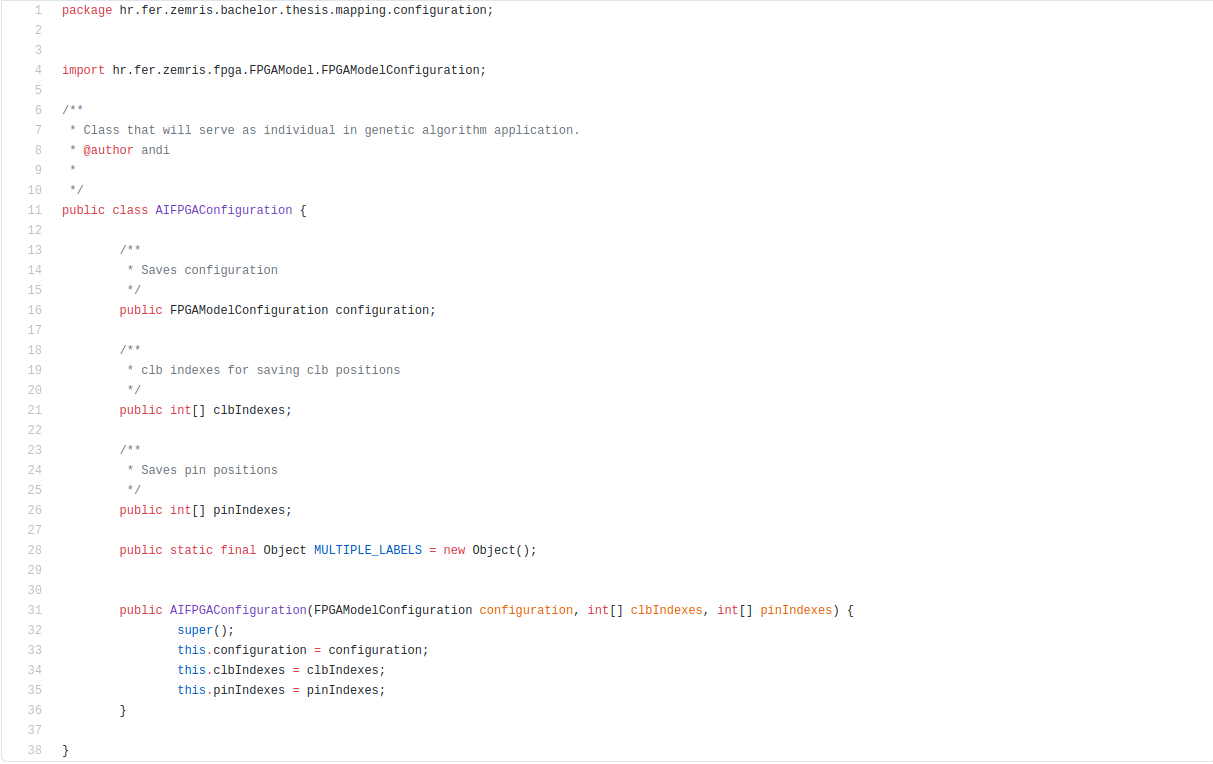
\includegraphics[width=18cm]{slike/AIFPGAConf.png}
		\caption{AIFPGAConfiguration jedinka genetskog algoritma}
		\label{fig:ai-fpga}
	\end{figure}
	
	
	Ona sadrži polja cijelih brojeva \emph{clbIndexes} i \emph{pinIndexes}. \\ \emph{ClbIndexes} je polje određeno brojem CLB-ova koji su nam na raspolaganju u FPGA modelu. U ovom radu koristio sam dva pristupa, jedan u kojem je očuvana različitost svih CLB pozicija te drugi slobodniji pristup kod kojeg su se mogli naći duplikati u konfiguraciji, ali se kasnije kažnjavaju preko funkcije dobrote. 
	
	\subsubsection{Clb pozicije}
	
	Jedna validna postavka polja \emph{clbIndexes} izgleda ovako: 
	
	\begin{table}[htb]
		\caption{\emph{clbIndexes}}
		\label{clbIndexes}
		\centering
		\begin{tabular}{|c | c | c | r|} \hline
			1 & 2 & 0 & 3 \\ \hline
		\end{tabular}
	\end{table}
	
	Ovakvom postavkom događa se sljedeće: na poziciji 1 u stvarnom fizičkom modelu FPGA sklopa nalazi se onaj CLB koji se dekompozicijom našao na poziciji 0 u logičkom modelu, na poziciji 2 je CLB koji se u logičkom modelu našao na poziciji 1 itd. \\
	
	\subsubsection{Pin pozicije}
	
	Slično izgleda i polje \emph{pinIndexes}. Kod njega se prvih \emph{m} indexa koristi za ulaze i redom se postavljaju svaka od \emph{m} ulaznih varijabli, a zatim sljedećih \emph{n} za izlaze. Moguće je da neki od pinova ostane neiskorišten, npr. ako imamo četiri ulazne varijable, tri izlazne i osam pinova ukupno, na njemu se neće generirati nikakav signal. 
	
	
	\begin{table}[htb]
		\caption{\emph{pinIndexes}}
		\label{pinIndexes}
		\centering
		\begin{tabular}{|c | c | c | c| c | c | c | c |} \hline
			4 & 5 & 7 & 0 & 2 & 1 & 6 & 3 \\ \hline
		\end{tabular}
	\end{table}
	
	Ako iskoristimo prijašnji primjer s četiri ulaza, tri izlaza i jednim neiskorištenim pinom onda takva konfiguracija \emph{pinIndexes} na pinove redom postavlja labele (pretpostavka je da su ulazne varijable redom A, B, C, D te izlazne F, G, H):
	
	\begin{table}[htb]
		\caption{\emph{pinLabels}}
		\label{pinLabels}
		\centering
		\begin{tabular}{|c | c |} \hline
			0 & D \\ \hline
			1 & G \\ \hline
			2 & F \\ \hline
			3 & - \\ \hline
			4 & A \\ \hline
			5 & B \\ \hline
			6 & H \\ \hline
			7 & C \\ \hline
		\end{tabular}
	\end{table}
	
	Osim ova dva polja \textbf{\emph{AIFPGAConfiguration}} razred agregira \textbf{\emph{FPGAModelConfiguration}} razred. 
	
	\begin{figure}[!htb]
		\centering
		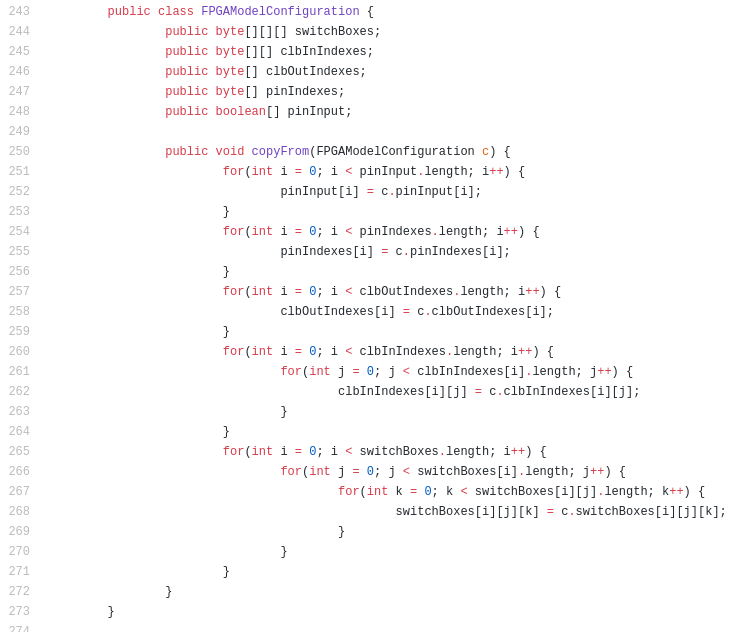
\includegraphics[width=18cm]{slike/FPGAModelConf.png}
		\caption{FPGAModelConfiguration razred, dio jedinke}
		\label{fig:fpga-model-conf}
	\end{figure} 
	
	\subsubsection{Prospojna kutija}
	
	Prvo što ćemo opisati kod ovog razreda jest konfiguracija prospojne kutije. One su definirane kao 3D polje gdje je jedna dimenzija određena brojem prospojnih kutija, a druge dvije dimenzije su veličine 4*broj žica u jednom snopu. Razlog zašto broj množimo s 4 je zato što prospojna kutija može spajati do 4 susjedna snopa žica, a 2D je polje zato što su veze usmjerene, a ne dvosmjerne pa je primjerice vezu od žice 2 jednog snop do žice 1 drugog snopa potrebno zapisati na dva mjesta. U svakom od \emph{n} prospojnih kutija nalazi se 2D polje bajtova, a u svako od polja može biti upisano 0, 1 ili 2. Ako je upisana 0, onda spoj ne postoji. Ako je upisana 1 to znači da spoj prima signal na toj žici, a svaka žica može primiti najviše jedan signal iz prospojne kutije. Ako je upisana 2 onda spoj šalje signal iz te žice pa je žica izlazna. Iz ovdje navedenih svojstava možemo izvesti zaključak kako je validna konfiguracija prospojne kutije ona koja u svakom retku ima najviše jednu 1 ili više 2 i ako je na mjestu [j][k] upisana 1 onda na poziciji [k][j] mora biti upisana 2 i obrnuto te ako je na [j][k] = 0 onda je i na [k][j] = 0. Također, žice iz istog snopa ne smiju biti povezane.
	
	
	\begin{table}[htb]
		\caption{\emph{Validna konfiguracija prospojne kutije u kojoj se snop žica sastoji od samo jedne žice.}}
		\label{swConfValid}
		\centering
		\begin{tabular}{|c|c|c|c|} \hline
			0 & 1 & 0 & 0 \\ \hline
			2 & 0 & 0 & 2 \\ \hline
			0 & 0 & 0 & 0 \\ \hline
			0 & 1 & 0 & 0 \\ \hline
		\end{tabular}
	\end{table}
	
	
	\begin{table}[!htb]
		\caption{\emph{Neispravna konfiguracija prospojne kutije u kojoj se snop žica sastoji od samo jedne žice. Ne može se dogoditi da jedna žica prima više signala (redak 0) te da jedna žica istovremeno šalje i prima signal (redak 3) }}
		\label{swConfInvalid}
		\centering
		\begin{tabular}{|c|c|c|c|} \hline
			0 & 1 & 0 & 1 \\ \hline
			2 & 0 & 0 & 2 \\ \hline
			0 & 0 & 0 & 0 \\ \hline
			2 & 1 & 0 & 0 \\ \hline
		\end{tabular}
	\end{table}
	
	\subsubsection{Ostali podatkovni članovi}
	
	\textbf{\emph{FPGAModelConfiguration}} sadržava još i \emph{clbInIndexes}, \emph{clbOutIndexes} i \emph{pinIndexes}, a svi oni pamte istu stvar: s koje od n žica, ako je n broj žica u snopu, prihvaćaju signal i ako je riječ o CLB-u - prosljeđuju dalje.
	
	\section{Algoritmi}
	
	Slijedi opis algoritama koji se spominju u završnom radu. Najprije opišimo dijelove koji koriste svi algoritmi.
	
	\subsubsection{Čistači}
	
	Svaki algoritam koji koristi takvo križanje ili takvu mutaciju koja može stvoriti neispravnu verziju prospojne kutije, koristi čistače. 
	
	\paragraph{Jednostavni čistač}
	
	Jednostavni čistač \textbf{\emph{SimpleSwitchBoxCleaner}} sve invalidne spojeve, postavlja na 0. Neispravna konfiguracija prospojne kutije je ona u kojoj je konfiguracija prospojne kutije takva da je pozicija [j][k] = 1, a pozicija [k][j] != 2 i obrnuto. U drugom slučaju je spoj već definiran kao izlazni i pokušava se redefinirati kao ulazni i obrnuto te zadnja mogućnost u kojoj spoj već prima signal s neke žice pa po definiciji ne smije primati signal s neke druge žice. 
	
	\paragraph{Napredniji čistač}
	
	Napredniji čistač \textbf{\emph{AdvancedSwitchBoxCleaner}} pokušava zamijeniti pozicije [j][k] i [k][j] i time eliminirati greške navedene kao drugi slučaj u prethodnom poglavlju.
	
	\subsection{Inicijalizatori i nasumični kreatori}
	
	Inicijalizator koristi \textbf{\emph{AIFPGAConfigurationRandomizer}} koji je zadužen za početno generiranje populacije. Radi tako da generira jednu po jednu jedinku koristeći pritom postavljene startne postavke:
	
	\begin{enumerate}
		\item U svakoj prospojnoj kutiji napravi se m validnih spojeva gdje je m nasumični broj iz intervala $[1, dohvatiMaxBrojVezaZaProspKutiju()]$. Maksimalan broj veza koji se može napraviti u svakoj prospojnoj kutiji je 3. 
		\item ClbInIndexes, clbOutIndexes i pinIndexes iz FPGAModelConfiguration se generiraju potpuno nasumično. 
		\item clbIndexes i pinIndexes su nasumični različiti brojevi. 
	\end{enumerate}
	
	
	\subsection{SV66}
	\label{SV66}
	
	Ovaj algoritam koristi napredni čistač prospojne kutije, križanje \emph{ValidCrosser}, \emph{SwapMutation} koji su opisani u poglavlju \ref{EndMutation} te proporcionalnu selekciju. Koristi se eliminacijski algoritam na način da je omogućen elitizam, a nova se jedinka stavlja na mjesto najlošije u roditeljskoj populaciji.
	
	\subsection{SV70}
	\label{SV70}
	
	Koristi sve iste dijelove kao i \ref{SV66}, samo što je ova verzija generacijski elitistički algoritam.
	
	\subsection{SV16}
	\label{SV16}
	
	Ova verzija algoritma koristi jednostavni čistač prospojnih kutija, vjerojatnosnu mutaciju kojoj se parametar $\alpha$ može proizvoljno podesiti te križanje s jednom točkom prijeloma. Primijetimo da ova verzija algoritma ne radi stalno s validnim konfiguracijama, nego je primjerice moguće da postoje duplikati u polju \emph{clbIndexes} koje bi, po definiciji, trebalo sadržavati sve različite vrijednosti. Po načinu rada ovo je eliminacijski genetski algoritam s jednostavnom troturnirskom selekcijom u koji je ugrađen elitizam.  
	
	\subsection{SV31}
	
	Eksperimentalno, iz nekih sam algoritama maknuo mutaciju. SV31 algoritam je jedan od takvih. Koristi jednostavni čistač prospojnih kutija i uniformno križanje.
	Možemo ga kategorizirati kao generacijski algoritam u koji nije ugrađen elitizam. 
	
	
	
	\subsection{Križanja i mutacije}
	
	\subsubsection{Križanje aritmetičkom sredinom}
	
	
	Tijekom rada algoritama primijećeno je kako križanje u kojem se za svaki gen računa aritmetička sredina ne daje dobre rezultate. Ako malo razmislimo o tome što koji gen jedinke predstavlja onda shvaćamo zašto je to tako. Uzmimo za primjer polje \emph{clbInIndexes}. To polje pamti pozicije žica s kojih se prima signal kod CLB sklopa. Pretpostavimo da su konfiguracije polja \emph{clbInIndexes} dvije jedinke ovakve:
	
	\begin{table}[H]
		\caption{\emph{Konfiguracija \emph{clbInIndexes} prve jedinke. Pretpostovljamo da postoji osam dvoulaznih CLB sklopova.}}
		\label{chromoClbIndex1}
		\centering
		\begin{tabular}{|c|c|c|c|} \hline
			0 & 1 \\ \hline
			2 & 1 \\ \hline
			2 & 1 \\ \hline
			2 & 2 \\ \hline
			0 & 0 \\ \hline
			1 & 2 \\ \hline
			2 & 1 \\ \hline
			2 & 2 \\ \hline
		\end{tabular}
	\end{table}
	
	\begin{table}[H]
		\caption{\emph{Konfiguracija \emph{clbInIndexes} druge jedinke. Pretpostovljamo da postoji osam dvoulaznih CLB sklopova i da se snop sastoji od 3 žice. }}
		\label{chromoClbIndex2}
		\centering
		\begin{tabular}{|c|c|c|c|} \hline
			2 & 1 \\ \hline
			1 & 2 \\ \hline
			0 & 2 \\ \hline
			1 & 1 \\ \hline
			0 & 1 \\ \hline
			2 & 0 \\ \hline
			1 & 1 \\ \hline
			1 & 2 \\ \hline
		\end{tabular}
	\end{table} 
	
	Nakon križanja, konfiguracija jedinke djeteta izgledati će ovako:
	
	\begin{table}[H]
		\caption{\emph{Konfiguracija \emph{clbInIndexes} djeteta. Pretpostovljamo da postoji osam dvoulaznih CLB sklopova i da se snop sastoji od 3 žice. }}
		\label{chromoClbIndexChild}
		\centering
		\begin{tabular}{|c|c|c|c|} \hline
			1 & 1 \\ \hline
			1 & 1 \\ \hline
			1 & 1 \\ \hline
			1 & 1 \\ \hline
			0 & 0 \\ \hline
			1 & 1 \\ \hline
			1 & 1 \\ \hline
			1 & 2 \\ \hline
		\end{tabular}
	\end{table}
	
	Prva stvar koja upada u oči jest da imamo jako puno parova samih jedinica. Prokomentirajmo zašto je to tako. \\
	Naime, u ovakvom FPGA modelu postoji 9 različitih parova roditelja pozicija i oni su redom: 00, 01, 02, 10, 11, 12, 20, 21 i 22. U 55.56\% slučajeva rezultat aritmetičke sredine roditeljskog para biti će upravo 1, u 33.33\% slučajeva rezultat će biti 0 dok je vjerojatnost da se očuva gen koji koristi pozicija 2 za dobivanje ulaznog signala jednaka 11.11\%. \\ 
	Osim matematike, razmišljanjem o problemu uviđamo kako genetskom algoritmu informacija da iz roditeljskog para pozicija npr. 02 nastaje gen 1 ne može puno pomoći. 
	
	
	\subsubsection{Završno križanje}
	\label{ValidCrosser}
	
	Nakon dugog eksperimentiranja uočene su neke stvari koje bi mogle pomoći u stvaranju kvalitetne jedinke te su implementirane kroz križanje i mutaciju. Križanje \emph{clbIndexes} i \emph{pinIndexes} se obavlja na način da se sa 50\%-tnom vjerojatnošću odabere jedinka od koje će se preuzeti gen, ali se on uzima samo ako ga je moguće uzeti odnosno ako taj gen već ne postoji. Inače se uzima gen druge jedinke.
	
	
	\begin{figure}[H]
		\centering
		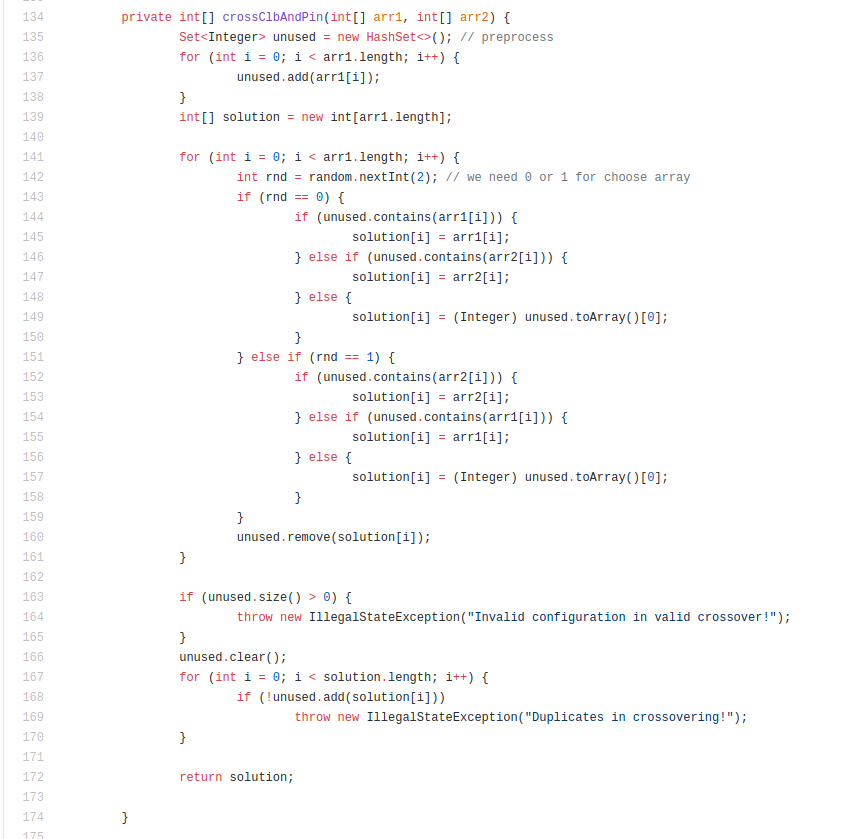
\includegraphics[width=18cm]{slike/crossClbAndPin.png}
		\caption{Križanje clb i pin pozicija.}
		\label{fig:clb-and-pin-positions}
	\end{figure} 
	
	Pozicije žica s kojih se uzima signal kod CLB sklopa i pinova, odnosno pozicija na koju se šalje križaju se običnim uniformnim križanjem. 
	
	\begin{figure}[H]
		\centering
		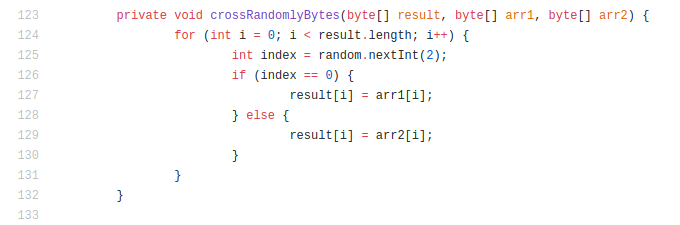
\includegraphics[width=18cm]{slike/crossRandomlyBytes.png}
		\caption{Uniformno križanje pozicija veza.}
		\label{fig:uniform-connection-crossing}
	\end{figure} 
	
	S obzirom da su prospojne kutije najkompliciraniji dio našeg sustava, kod njih i imamo najsloženije križanje. Prije je spomenuto kako kažnjavamo previše veza u jednoj prospojnoj kutiji te kako početni konfigurator stvara ograničeni broj veza. Kada bismo koristili uniformno križanje i kod prospojnih kutija kroz npr. 10000 generacija njihov bi se genetski materijal jednostavno izgubio. Zato se, u konfiguracijama u kojima algoritam bira između veze u jednoj jedinki i nepostojeće veze u drugoj, sa 70\% vjerojatnošću bira veza. Ako obje konfiguracije sadrže veze onda koristimo uniformno križanje gena. 
	
	\begin{figure}[H]
		\centering
		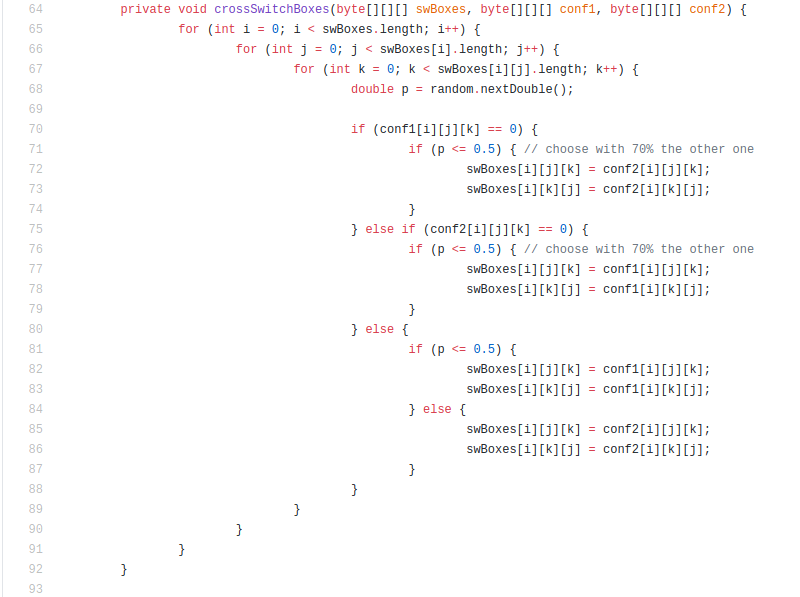
\includegraphics[width=18cm]{slike/crossSwBoxes.png}
		\caption{Križanje prospojnih kutija.}
		\label{fig:sw-boxes-crossing}
	\end{figure} 
	
	\subsubsection{Završna mutacija}
	\label{EndMutation}
	
	Mutacija je genetski operator kojemu je posvećeno najviše pažnje. Izvedena je na način da se pozicije s kojih se prima ulazni signal zarotiraju ulijevo pa tako ako jedinka ima pozicije 01, nakon mutacije će imati 10. S time se želi isprobati još jedna konfiguracija prije promjene genetskog materijala kod djeteta jer možda je konfiguracija prospojne kutije takva da ima dobre veze, ali su samo signali zamijenjeni.  
	
	\begin{figure}[H]
		\centering
		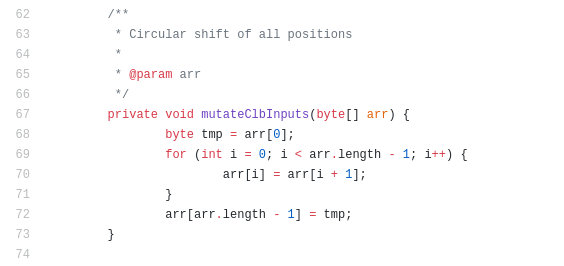
\includegraphics[width=18cm]{slike/circularShift.png}
		\caption{Mutiranje ulaznih signala.}
		\label{fig:sw-boxes-inputs-mutation}
	\end{figure} 
	
	Pozicije CLB sklopova i ulazno/izlazne veze mutiraju na način da se kod njih primijeni postupak kao u poglavlju \ref{SwapMutation}.
	
	\begin{figure}[H]
		\centering
		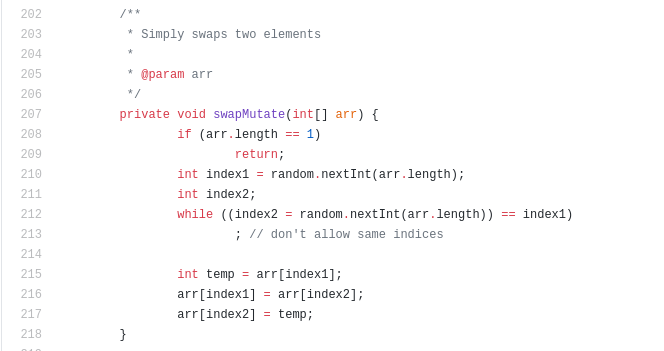
\includegraphics[width=18cm]{slike/swapMutate.png}
		\caption{Vjerojatnosna mutacija pozicija. }
		\label{fig:sw-boxes-mutation}
	\end{figure} 
	
	Sljedeći pseudokod objašnjava postupak izmjene gena prospojnih kutija: 
	
	\begin{figure}[H]
		\centering
		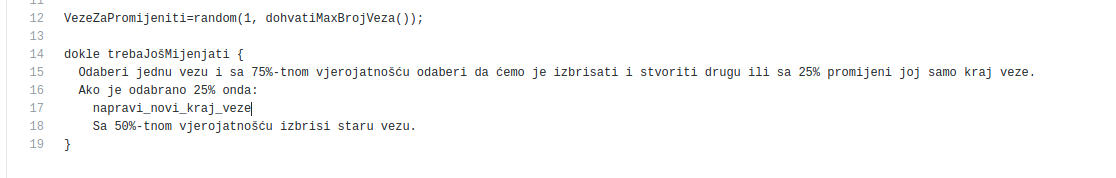
\includegraphics[width=18cm]{slike/pseudokod.png}
		\caption{Promjena genetskog materijala prospojnih kutija.}
		\label{fig:pseudokod-prospojne}
	\end{figure} 
	
	\subsection{Funkcija dobrote}
	
	Svaki genetski algoritam ima svoja nužna ograničenja koja se brinu o tome da zadovoljavaju svojstva sustava. Ovaj sustav podrazumijeva dva nužna ograničenja koja svako rješenje mora zadovoljiti da bi bilo iskoristivo:
	
	\begin{enumerate}
		\item Ulazi na svaki CLB sklop moraju biti točno oni koji su dobiveni dekompozicijom logičkih funkcija.
		\item Izlazi svakog CLB sklopa moraju biti odvedeni na točno onaj UI spoj (eng. \emph{Pin}) koji je specificiran u tekstualnoj datoteci kojom zadajemo logički model.
	\end{enumerate}
	
	\subsubsection{Hibridna funkcija dobrote}
	
	Prva verzija algoritma radila je s hibridnom funkcijom dobrote u kojoj su se dobre stvari nagrađivale, a loše kažnjavale. Takav se model nije pokazao dobrim iz dva razloga:
	\begin{enumerate}
		\item Nijedan od 70 inačica algoritma ni nakon $\approx100000$ pokretanja nije pronašao rješenje ni za najjednostavniji primjer.
		\item Vrlo je teško bilo pratiti da li je najbolja jedinka kvalitetno rješenje ili ne zbog velikog broja mogućnosti s kojim se moglo doći do tog rezultata. 
	\end{enumerate}
	
	Način vrjednovanja može se iščitati iz tablice \ref{HibridnaFunkcija}
	
	
	\begin{table}[htb]
		\caption{\emph{Hibridna funkcija}}
		\label{HibridnaFunkcija}
		\centering
		\begin{tabular}{|c | c|} \hline
			Točan ulaz na CLB sklopu & +30 \\ \hline
			\makecell{Krivi tip na ulazu CLB sklopa, \\ npr. ništa nije dovedeno ili doveden je izlaz CLB sklopa, a treba nam pin} & -20 \\ \hline
			Krivi ulaz na CLB sklopu, ali dobar tip& -10 \\ \hline
			Izlaz iz CLB sklopa se odvodi na traženi pin & +30 \\ \hline
			Izlaz iz CLB sklopa se ne odvodi na traženi pin & -10 \\ \hline 
			Izlaz iz CLB sklopa se odvodi na traženi pin i na još neke & -5
		\end{tabular}
	\end{table}
	
	\begin{figure}[H]
		\centering
		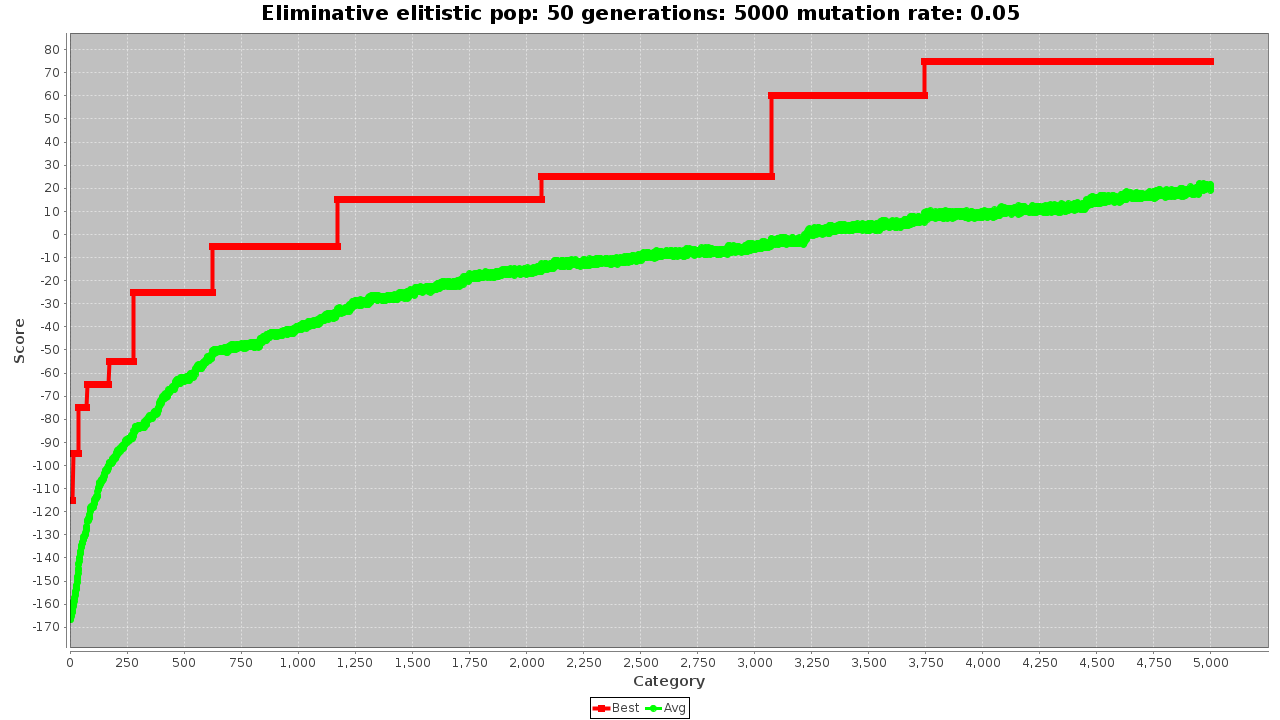
\includegraphics[width=18cm]{slike/SV66Hibrid.png}
		\caption{Primjer funkcije dobrote za algoritam SV66}
		\label{fig:sv66-alg-hibrid}
	\end{figure} 
	
	Iz slike \ref{fig:sv66-alg-hibrid} vidimo kako prosječna vrijednost funkcije dobrote raste što upućuje na to da model hibridne funkcije kao takav ima smisla. Crvena linija prati vrijednost funkcije dobrote najbolje jedinke i taj je graf rastući zbog ugrađenog svojstva elitizma. Primijetimo da svaki skok (stepenica) na crvenoj liniji znači da je pronađeno nešto što naš model nagrađuje ili kažnjava pa nije kaznio. Vrijednosti skokova možemo protumačiti uz pomoć tablice \ref{HibridnaFunkcija}. Vidimo da je do 250. generacije sustav uspio pronaći 3 točna ulaza i/ili izlaza te 2 takva ulaza i/ili izlaza koji imaju dovedene točne tipove, ali krive signale (npr. doveden je ulaz A, a trebao je biti B). Primijetimo da, iako je to nešto što je krivo i ne odgovara našoj definiciji sustava, to ne bi trebalo jako kažnjavati jer u principu mi želimo iskoristiti veze prospojne kutije te jedinke, a samo moramo promijeniti vrijednost ulazne varijable. No, to možemo i samo premetanjem u \emph{pinIndexes} pa bi takvu jedinku genetski algoritam trebao puno lakše pronaći, nego stvarati potpuno novu konfiguraciju prospojne kutije. 
	
	Pogledajmo kako se ponaša algoritam SV31. 
	
	\begin{figure}[H]
		\centering
		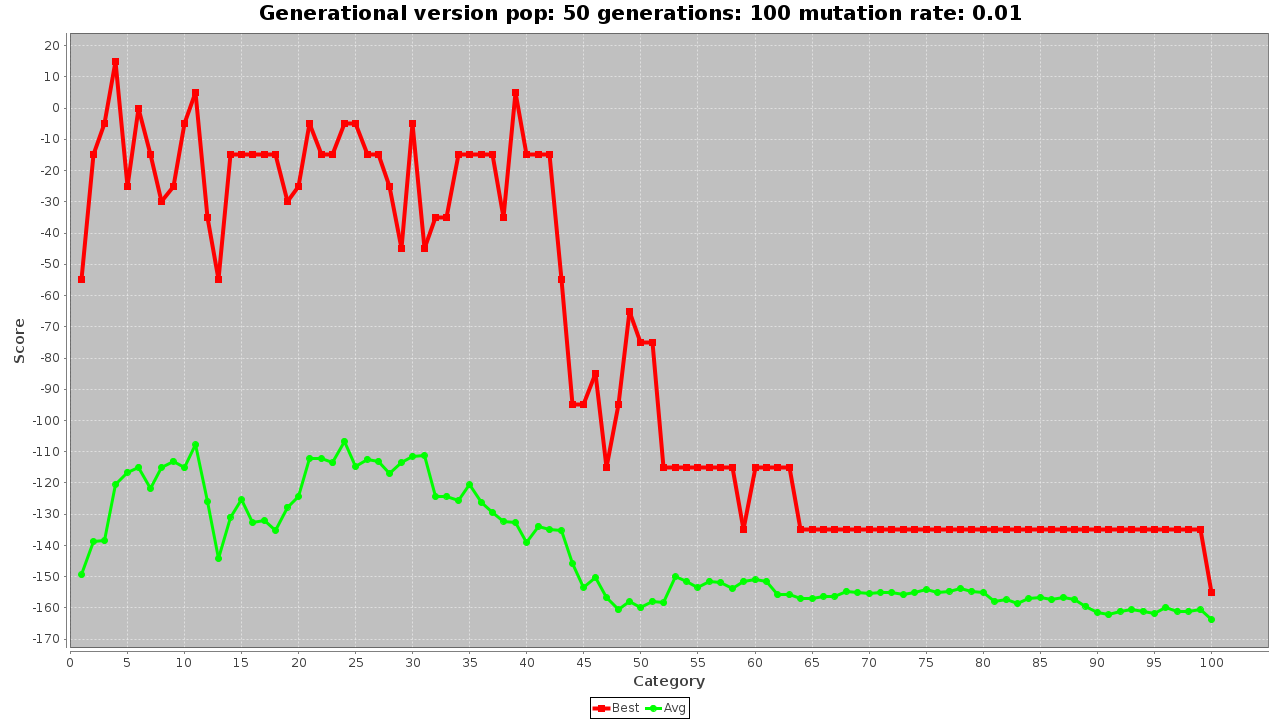
\includegraphics[width=18cm]{slike/SV31Hibrid.png}
		\caption{Primjer funkcije dobrote za algoritam SV31}
		\label{fig:sv31-alg-hibrid}
	\end{figure} 
	
	
	Odmah se vidi na prvu da algoritam nije dobar. Prvu stvar koju primjećujemo je skokovitost crvene linije koja nam prati najbolju jedinku kroz generacije i koja pri kraju rada algoritma doseže pad. No, s obzirom da u ovaj algoritam nije ugrađen elitizam, skokovitost nas ne čudi. Ono što stvarno pokazuje kako konvergencija algoritma zapravo i ne postoji je zelena linija koja prati prosječnu vrijednost dobrote kroz generacije. Primjećujemo da postoje intervali generacija na kojem ona raste, ali globalno gledajući, ona pada što upućuje na to da genetski algoritam zapravo nema pojma radi li nešto dobro ili loše.\\
	S obzirom da ne postoji nijedno istraživanje koje bi nam dalo za pravo zaključiti da je generacijski algoritam lošiji od eliminacijskog, zaključujemo da je sustav u kojem ne postoji mutacija loš te nije korišten u daljnjem radu. \\
	\textbf{Napomena: } Svi slučajevi koji se opisuju ovdje dobiveni su pokretanjem algoritama više stotina puta, a ovdje su uzeti primjeri koji najbolje oslikavaju ponašanje konkretnog algoritma.  
	
	Algoritam koji je najviše obećavao na početku bio je zapravo i najjednostavniji: SV16. 
	
	\begin{figure}[!htb]
		\centering
		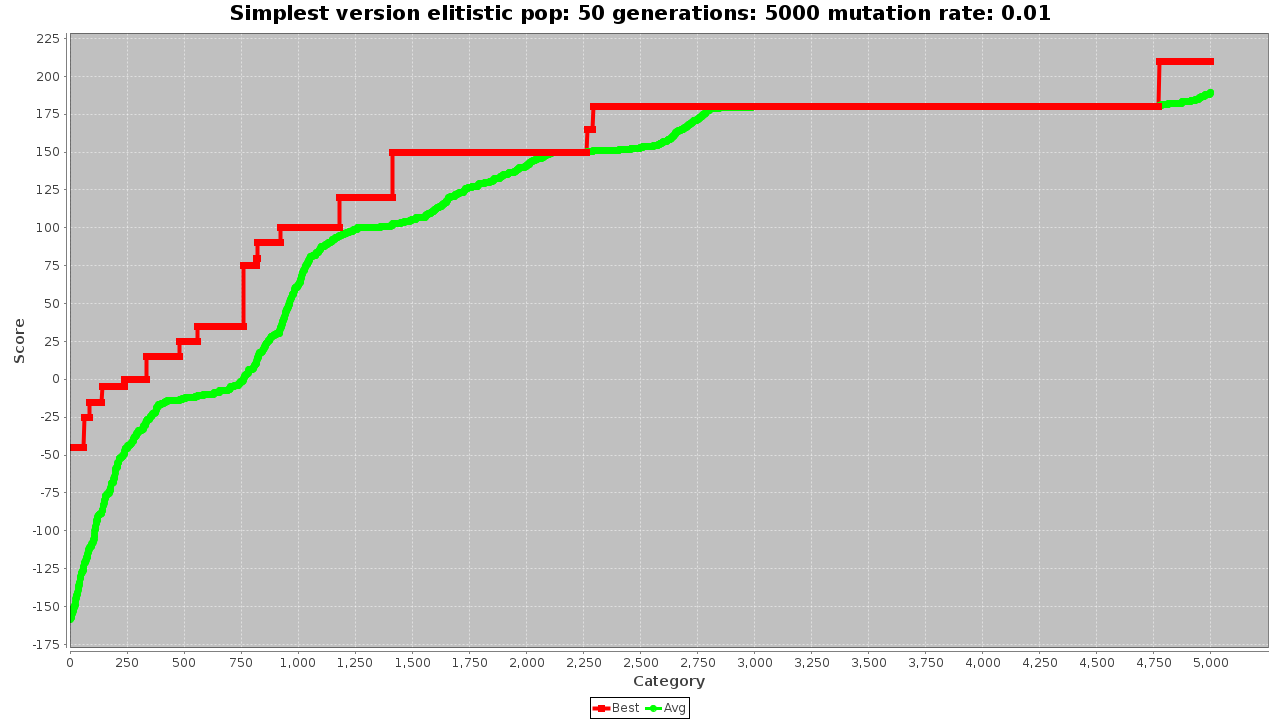
\includegraphics[width=18cm]{slike/SV16Hibrid.png}
		\caption{Primjer funkcije dobrote za algoritam SV16}
		\label{fig:sv16-alg-hibrid}
	\end{figure} 
	
	Iako je po samom principu rada vrlo sličan algoritmu SV66, pri gotovo svakom pokretanju algoritma, možemo uvidjeti kako postoji puno više manjih skokova kod najbolje dobrote jedinke, a prosječna dobrota raste puno brže, nego kod SV66. Zanimljivo, SV16 ne koristi nikakvu posebnu selekciju već, kao što je navedeno u \ref{SV16}, nasumično odabire tri jedinke, križa dvije od tri te dijete stavi na mjesto treće ako ima veću dobrotu. 
	
	\subsubsection{Neuspješna nadogradnja hibridne funkcije dobrote}
	
	Prije nego što zagazimo u kompliciraniji model kreiranja funkcije dobrote spomenimo još jedan korišteni pristup. Za vrijeme rada algoritma primijećeno je kako algoritam u puno slučajeva uspije na ispravan način dovesti izlaze CLB sklopa na pinove, ali nikada nije u stanju više od 5 ulaza ispravno posložiti. Pokušao sam kreirati takvu funkciju dobrote u kojoj svaki pronađeni ulaz donosi puno više, nego što krivi odnosi. Nagrada se tada za svaki točan ulaz povećavala s kvadratnim članom, a svaki krivi ulaz smanjivala s linearnim članom. Formula za n točnih i m krivih ulaza izgleda ovako: 
	
	\begin{equation}
		value=\sum_{i=1}^{n}i^2 - 5\ast \sum_{k=1}^{m}k
	\end{equation}
	
	Sve moguće kombinacije točnih/krivih ulaza zapisani su u tablici \ref{NadograđenaHibridnaFunkcija}: 
	
	\begin{table}[htb]
		\caption{\emph{Neuspješna nadogradnja hibridne funkcije dobrote}}
		\label{NadograđenaHibridnaFunkcija}
		\centering
		\begin{tabular}{|c | c | c|} \hline
			\thead{Točnih} & \thead{Krivih} & \thead{Vrijednost} \\ \hline
			8 & 0 & 204 \\ \hline
			7 & 1 & 135 \\ \hline
			6 & 2 & 76 \\ \hline
			5 & 3 & 25 \\ \hline
			4 & 4 & -20 \\ \hline
			3 & 5 & 61 \\ \hline
			2 & 6 & -100 \\ \hline
			1 & 7 & -139 \\ \hline
			0 & 8 & -175 \\ \hline
		\end{tabular}
	\end{table}
	
	Funkcija dobrote za izlaze modelirana je na isti način kao i za ulaze samo što su te vrijednosti skalirane s parametrom 0.5. Time sam želio postići da se jedinke s dobrim ulazima više koriste u reprodukciji novih, nego one s točnim izlazima. Nažalost, ni ovo nije dovelo do pronalaska nikakvih potpunih rješenja. 
	
	Jedan tipičan primjer kako je izgledala funkcija dobrote dok se koristio ovakav model(samo s drugim faktorima) prikazan je na slici \ref{fig:sv54-convergence}. 
	
	\begin{figure}[!htb]
		\centering
		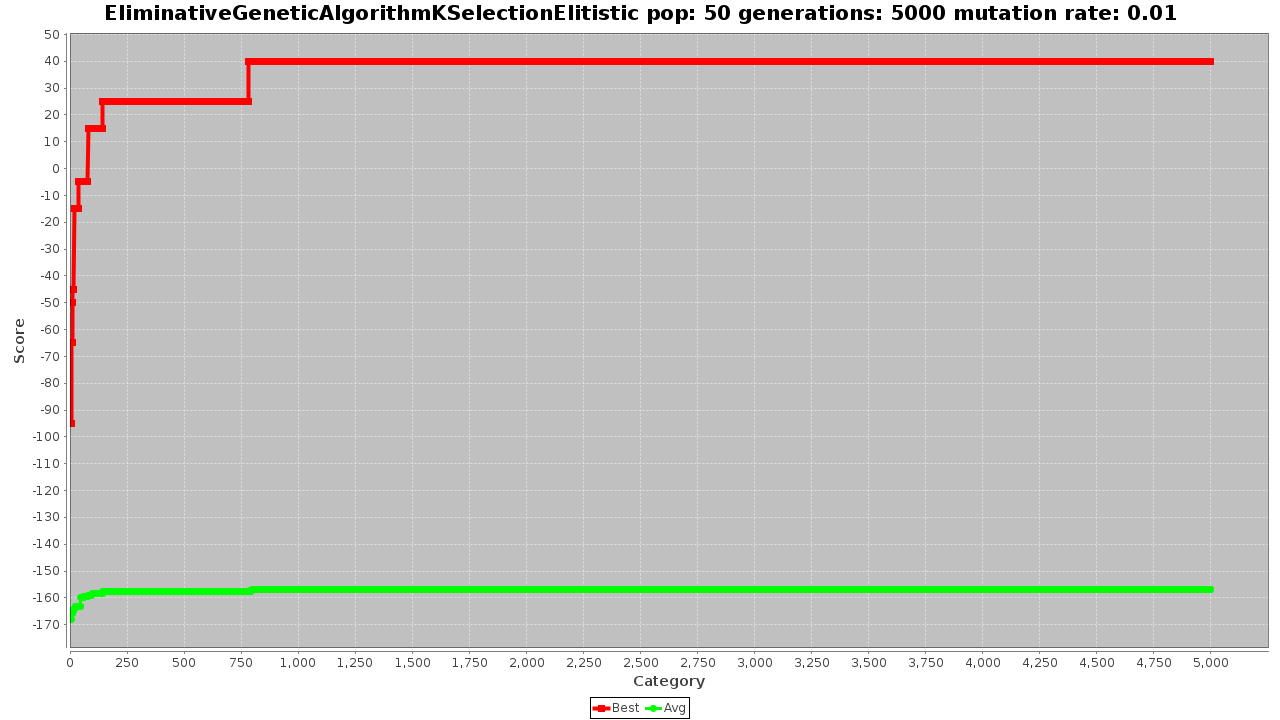
\includegraphics[width=18cm]{slike/SV54Convergence.png}
		\caption{Primjer preuranjene konvergencije}
		\label{fig:sv54-convergence}
	\end{figure} 
	
	Osim što primjećujemo da genetski algoritam malo toga pronalazi (ima malo skokova), zanimljivo je da sve novo algoritam pronađe do 1000. generacije. Takvu pojavu nazivamo preuranjena konvergencija, a radi se o tome da algoritam zapne u lokalnom optimumu i zbog premalo mutacije, odnosno u ovom slučaju zbog ne baš najsretnije funkcije dobrote, ne uspije pretražiti ostatak prostora rješenja. 
	
	\subsubsection{Smanjenje prostora pretraživanja stanja}
	
	Kako bismo olakšali posao genetskom algoritmu, sljedeći je korak bio smanjiti prostor pretraživanja. Pažljivi je čitatelj mogao primijetiti kako su se kod rubnih prospojnih kutija mogle naći veze koje su spajale dvije nepostojeće žice ili jednu nepostojeću s jednom postojećom žicom. Iz tog smo razloga nadogradili \textbf{\emph{AIFPGAConfigurationRandomizer}} te je od onda stvarao samo smislene veze u prospojnoj kutiji. Također su, mutacija i križanje doživjeli promjene te sada i oni prilikom reprodukcije djece, odnosno promjene genetskog materijala, stvaraju validne gene. 
	
	
	\begin{figure}[!htb]
		\centering
		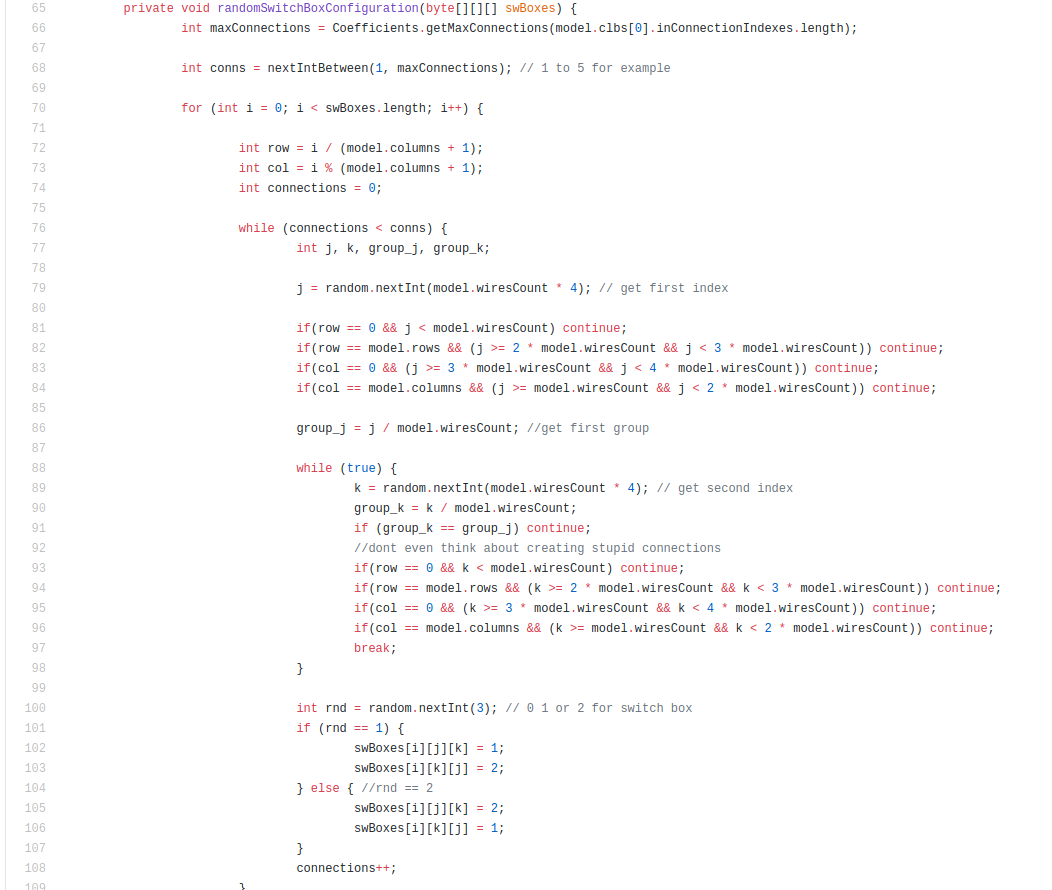
\includegraphics[width=18cm]{slike/noviRandomizer.png}
		\caption{Unaprijeđena verzija stvaranja konfiguracija prospojnih kutija}
		\label{fig:novi-random}
	\end{figure} 
	
	
	
	Sustav je kroz cijelo vrijeme bio unaprijeđivan na temelju uviđenih stvari koje nisu nužno bile krive, ali su vrlo brzo dovodile do jedinki koje nisu rješenja. Prvo što sam odlučio dodati u model jest informacija ima li i koliko ima gaženja signala u modelu. Ako pogledamo \ref{fig:arh-fpga} vidimo da je moguće da se više ulaza, više izlaza ili pak više ulaza i izlaza nađu na nekom CLB ulazu. Takva situacija nam je vrlo nepovoljna iz jednostavnog razloga što onda taj model ne može biti nikako ispravan i teško možemo bilo šta iskoristiti iz te jedinke za stvaranje nove. Odnosno preciznije je reći da bismo možda mogli i iskoristiti nešto, ali zbog nedeterminizma u mutaciji i križanju ne želimo riskirati i uzeti lošu stvar iz te jedinke u izgradnji nove. Upravo zato se taj slučaj kažnjava s vrlo velikim faktorom jer želimo da relativna proporcionalna selekcija s vrlo malom vjerojatnošću uzme takvu jedinku pri izgradnji djeteta. \\ 
	Osim toga, počeli smo razlikovati situacije u kojima na ulaze/pinove nije ništa dovedeno u odnosu na prijašnje situacije u kojima je jedini bio mogući krivi tip odnosno krivi signal. I ovakvo stanje želimo kazniti s velikim faktorom jer moramo mijenjati konfiguraciju prospojne kutije kod djeteta što je puno teži zadatak, a ne samo ulaze/izlaze. 
	
	
	\begin{figure}[H]
		\centering
		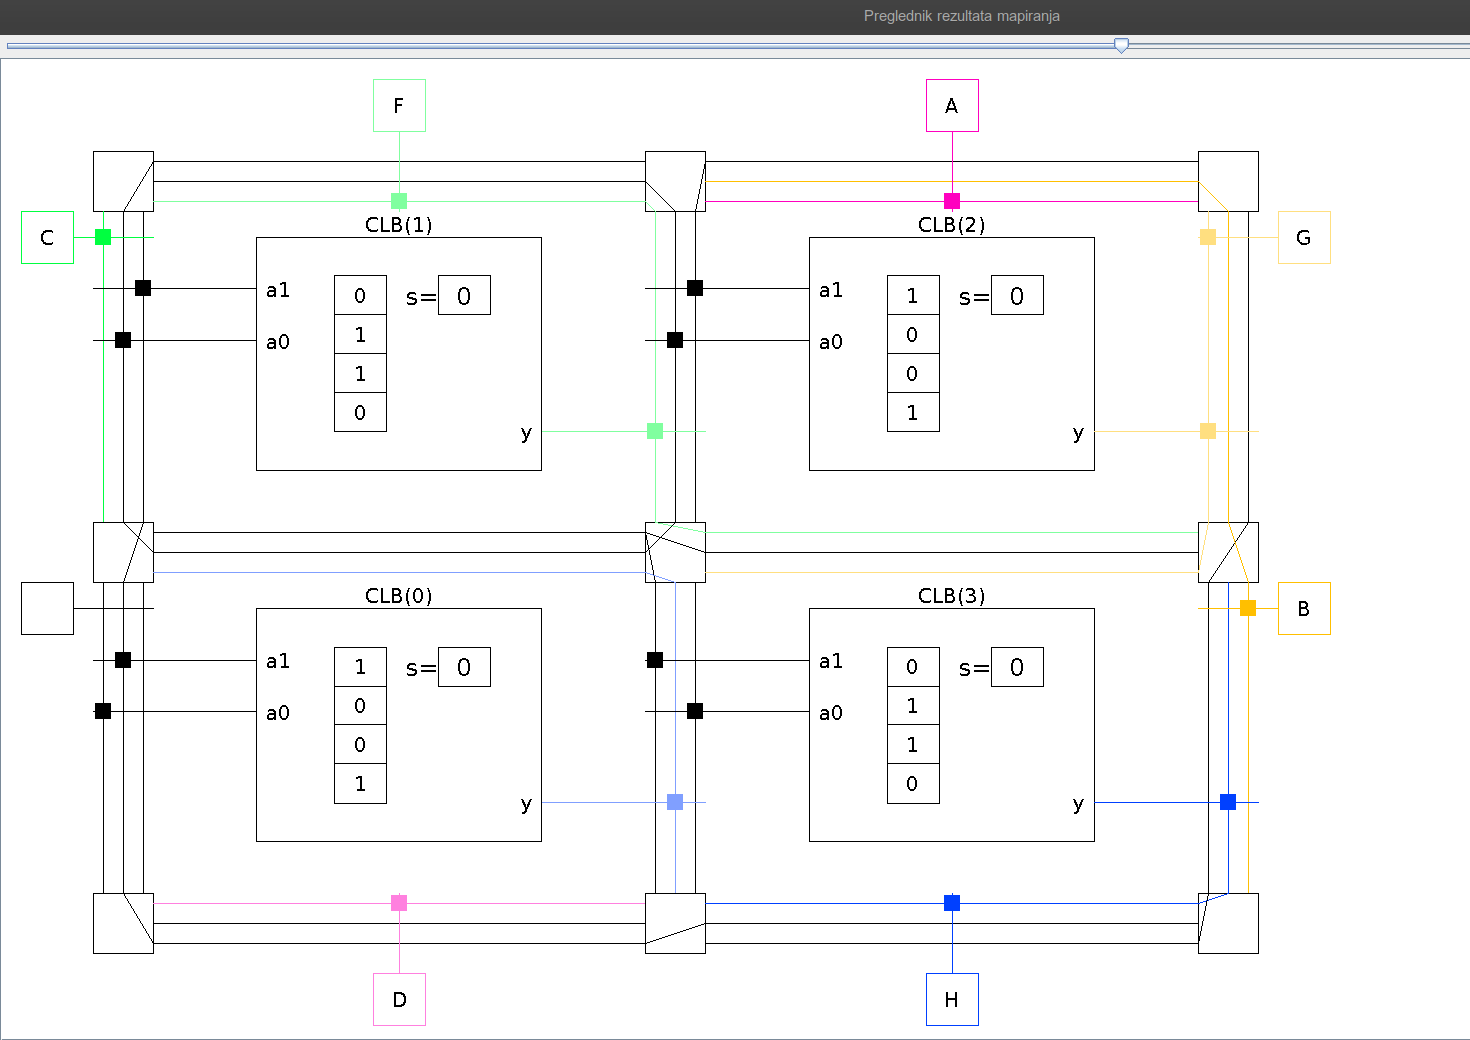
\includegraphics[width=18cm]{slike/blackLabel.png}
		\caption{Primjer rješenja u kojem genetski algoritam ne zna za prazan spoj. Crni kvadratići označavaju da nije nikakav signal doveden. }
		\label{fig:black-label}
	\end{figure} 
	
	
	
	\begin{figure}[H]
		\centering
		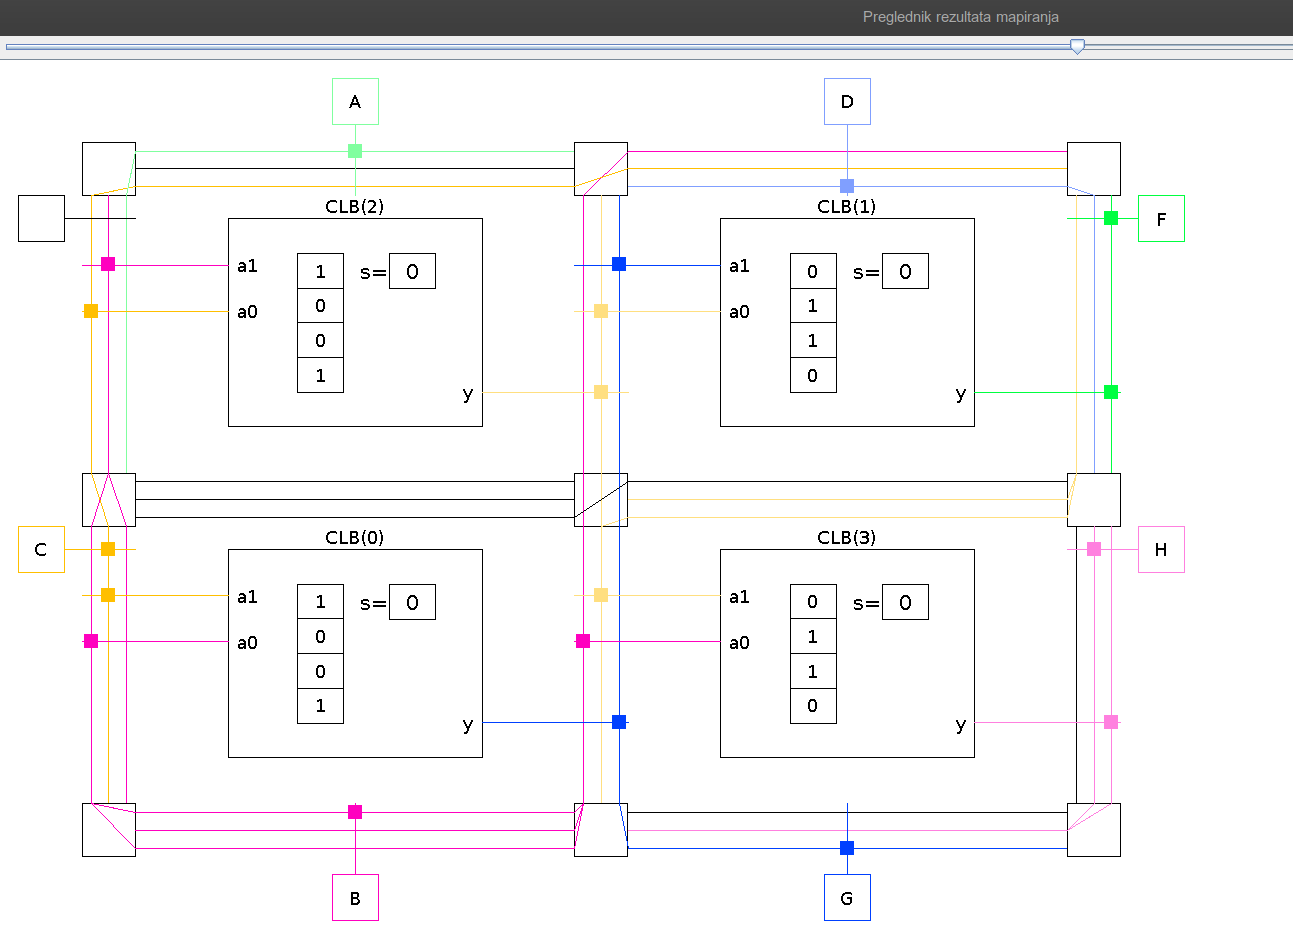
\includegraphics[width=18cm]{slike/withoutBlackLabel.png}
		\caption{Primjer rješenja u kojem genetski algoritam ne dopušta da se na ulaze ne dovodi nikakav signal.}
		\label{fig:black-label}
	\end{figure} 
	
	
	Kroz cijeli proces izgradnje funkcije dobrote fokus je bio na prospojnim kutijama. Naime, ako su one previše ili premalo toga spojile onda nije bilo šanse da druge strukture podataka "izvuču" algoritam iz zapinjanja. Stoga sam svaku prospojnu kutiju u kojoj su se nalazile više od tri veze počeo kažnjavati jer sam uvidio kako previše veza najčešće znači i gaženje signala. To je ipak, kažnjavano s malim faktorom jer iako ima previše veza, moguće je da su neke od njih korisne pa takve jedinke ne želimo u potpunosti eliminirati kao one kod kojih je već primijećeno gaženje signala. 
	
	
	
	\begin{figure}[H]
		\centering
		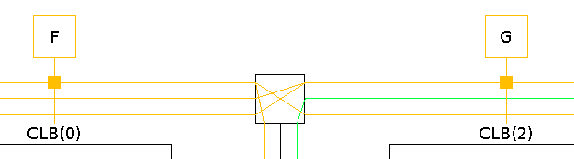
\includegraphics[width=18cm]{slike/isjecakPreviseVeza.png}
		\caption{Previše spojeva u prospojnoj kutiji na poziciji 1. Takva situacija često dovodi do gaženja signala. }
		\label{fig:previse-veza}
	\end{figure} 
	
	
	Još jedna stvar kod prospojnih kutija nije bila poželjna, a često je bila primijećena: kad god je jedna žica proslijedila signal na više od jedne žice u neki snop to je obično u startu značilo da ta jedinka ne sadržava kvalitetan genetski materijal.
	
	
	
	\begin{figure}[H]
		\centering
		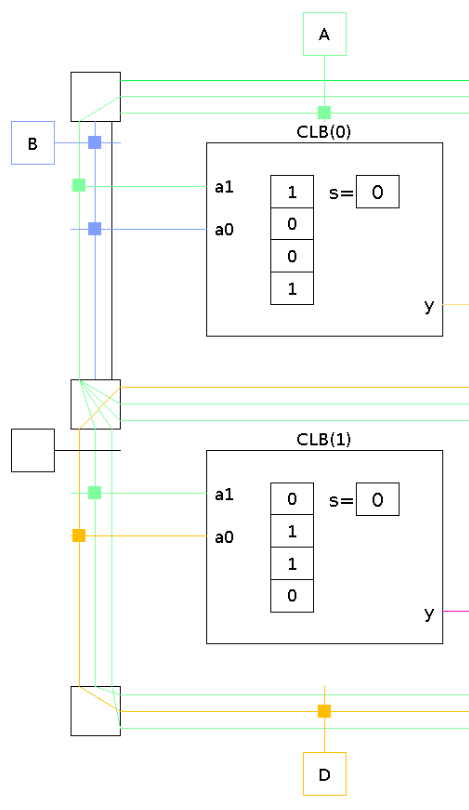
\includegraphics[width=10cm]{slike/isjecakSusjedneVeze.png}
		\caption{Signal B se prosljeđuje na više žica u istom snopu, ipak to u ovom slučaju nije problem. }
		\label{fig:susjedne-veze}
	\end{figure} 
	
	
	Razlog je što na niti jedan CLB sklop nikad nećemo dovoditi više istih ulaza pa jedinku kod koje je takav slučaj uočen, kažnjavamo. 
	
	Naravno, kao što je i problem ako imamo previše veza u nekoj prospojnoj kutiji, ako nemamo nijednu isto nije dobro pa svaki put kada je prospojna kutija prazna, dobroti jedinke dodamo kaznu. Takvo kažnjavanje nije zato jer nju ne želimo koristiti, moguće je da ona ima dobrih veza u drugim prospojnim kutijama koje nam trebaju, ali će ipak u većini slučajeva prazna prospojna kutija biti znak loše kvalitete rješenja. 
	
	
	\begin{figure}[H]
		\centering
		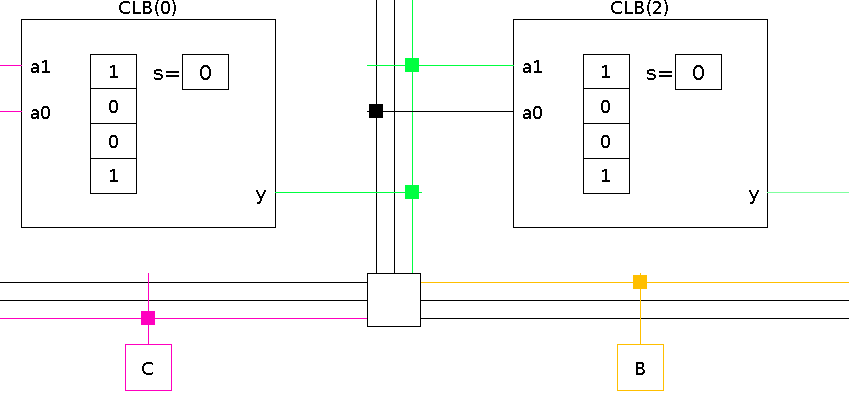
\includegraphics[width=18cm]{slike/isjecakPraznog.png}
		\caption{Iako ne nužno loš znak, prazna prospojna kutija često dovodi do zastoja signala na njegovom putu.}
		\label{fig:prazna-skatula-isjecak}
	\end{figure} 
	
	Dodavanjem ovih parametara u dobrotu funkcije došli smo do stanja u kojem prospojne kutije više manje imaju uvijek optimalan broj veza. Sljedeća situacija za koju smo uvidjeli da nije dobra i da bi je trebalo popraviti je ona u kojoj se signal s nekog ulaznog pin ne prosljeđuje na niti jednu susjednu prospojnu kutiju. U tom slučaju jedinka zapravo zaboravlja na taj ulaz pa će sigurno, gdje god bi se on trebao koristiti, tamo naći praznina ili krivi signal. 
	
	\begin{figure}[H]
		\centering
		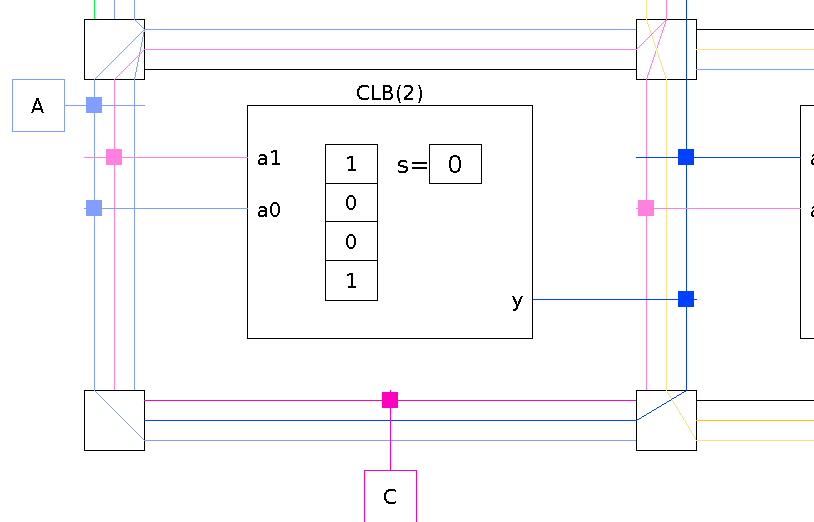
\includegraphics[width=18cm]{slike/isjecakCNikamo.png}
		\caption{Signal s UI spoja C se ne prosljeđuje ni kroz jednu od dvije prospojne kutije. }
		\label{fig:isjecak-c-nikamo}
	\end{figure} 
	
	
	\chapter{Eksperimentalni rezultati}
	
	\section{Opis}
	
	U ovom ću dijelu opisati koji su dosezi ovakvog sustava i koja su moguća poboljšanja trenutačnog sustava. Algoritam koji se tijekom rada pokazao najboljim je SV66 pa su svi primjeri iz ovog poglavlja rezultat njegovog rada. 
	
	\section{Rezultati}
	
	Sustav pronalazi rješenje u 100\% slučajeva kada mu je zadatak mapirati logički model s jednim CLB sklopom u fizički FPGA model s jednim CLB sklopom.
	
	
	\begin{figure}[H]
		\centering
		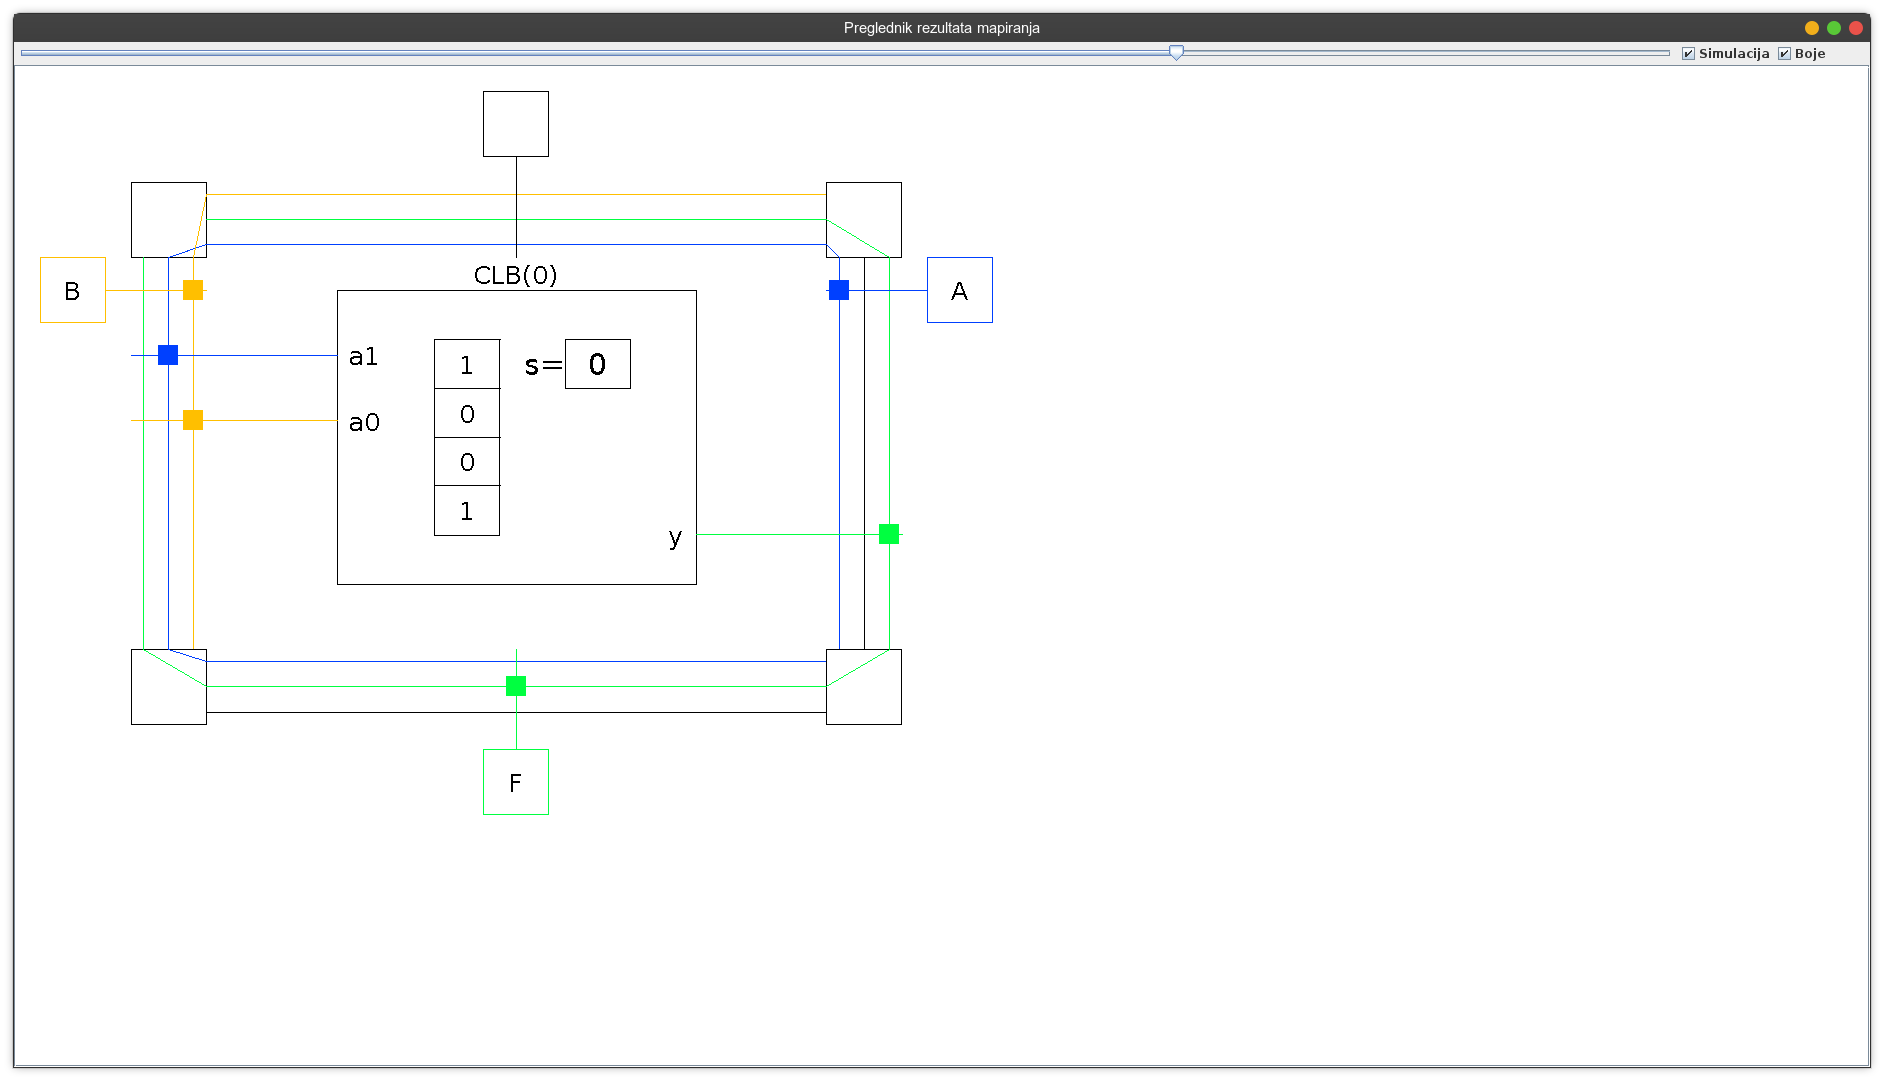
\includegraphics[width=15cm]{slike/1111.png}
		\caption{Sustav uvijek pronalazi rješenje kod kada je potrebno mapirati jedan CLB u fizički model.}
		\label{fig:1111-founded-img}
	\end{figure} 
		
		Primijećeno jest kako se sustav puno bolje ponaša kada ima zadane okomito postavljene CLB sklopove, nego kada su oni vodoravno postavljeni. Razlog tomu je što, ako imamo malo ulaznih žica tada će se u jako puno iteracija dogoditi da prvi CLB sklop svoj izlaz prosljeđuje na ulaz drugog. 
		
		
		Zadatak u kojem postoji više fizičkih CLB-ova, nego logičkih, sustav ne rješava uvijek. Iako se na prvu čini da bi sustav takvo rješenje trebao lakše pronaći, to nije tako. Naime, genetski algoritam sada barata s većom količinom potencijalnih informacija, a to što on mapira samo jedan logički sklop, samo olakšava provjeru je li rješenje pronađeno.
		Kako bismo smanjili prostor pretraživanja, u takvoj se situaciji ulazne i izlazne pozicije CLB sklopa drže na -1 pa se u tom dijelu signali uopće ne prosljeđuju. Time je postotak pronalaska rješenja povećan za 10\%.
		
		Iz tablice \ref{gen-alg-result} naravno vidimo da i sve što je zadatak mapiranja složeniji, to je i postotak pronalaska rješenja manji, a sustav ne pronalazi uopće rješenja za 4 i više CLB sklopa. 
		
		Zbog toga sam odlučio konstruirati eksperiment kojim ću pokazati da se taj sustav ipak kreće u dobrom smjeru. U tu sam svrhu kreirao logički zadatak u kojem se izlaz nultog sklopa šalje na drugi, a izlaz prvog na treći sklop. Kada bi ljudi rješavali takav problem intuicija nam govori kako je puno lakše dobro posložiti ulaze kada se nulti sklop nalazi prije drugog odnosno prvi sklop ispred trećeg, vodoravno gledano. To znači da su nam, od mogućih 4!=12 konfiguracija validne dvije, a prikazane su na slikama ispod.
		
		
		\begin{figure}[H]
			\centering
			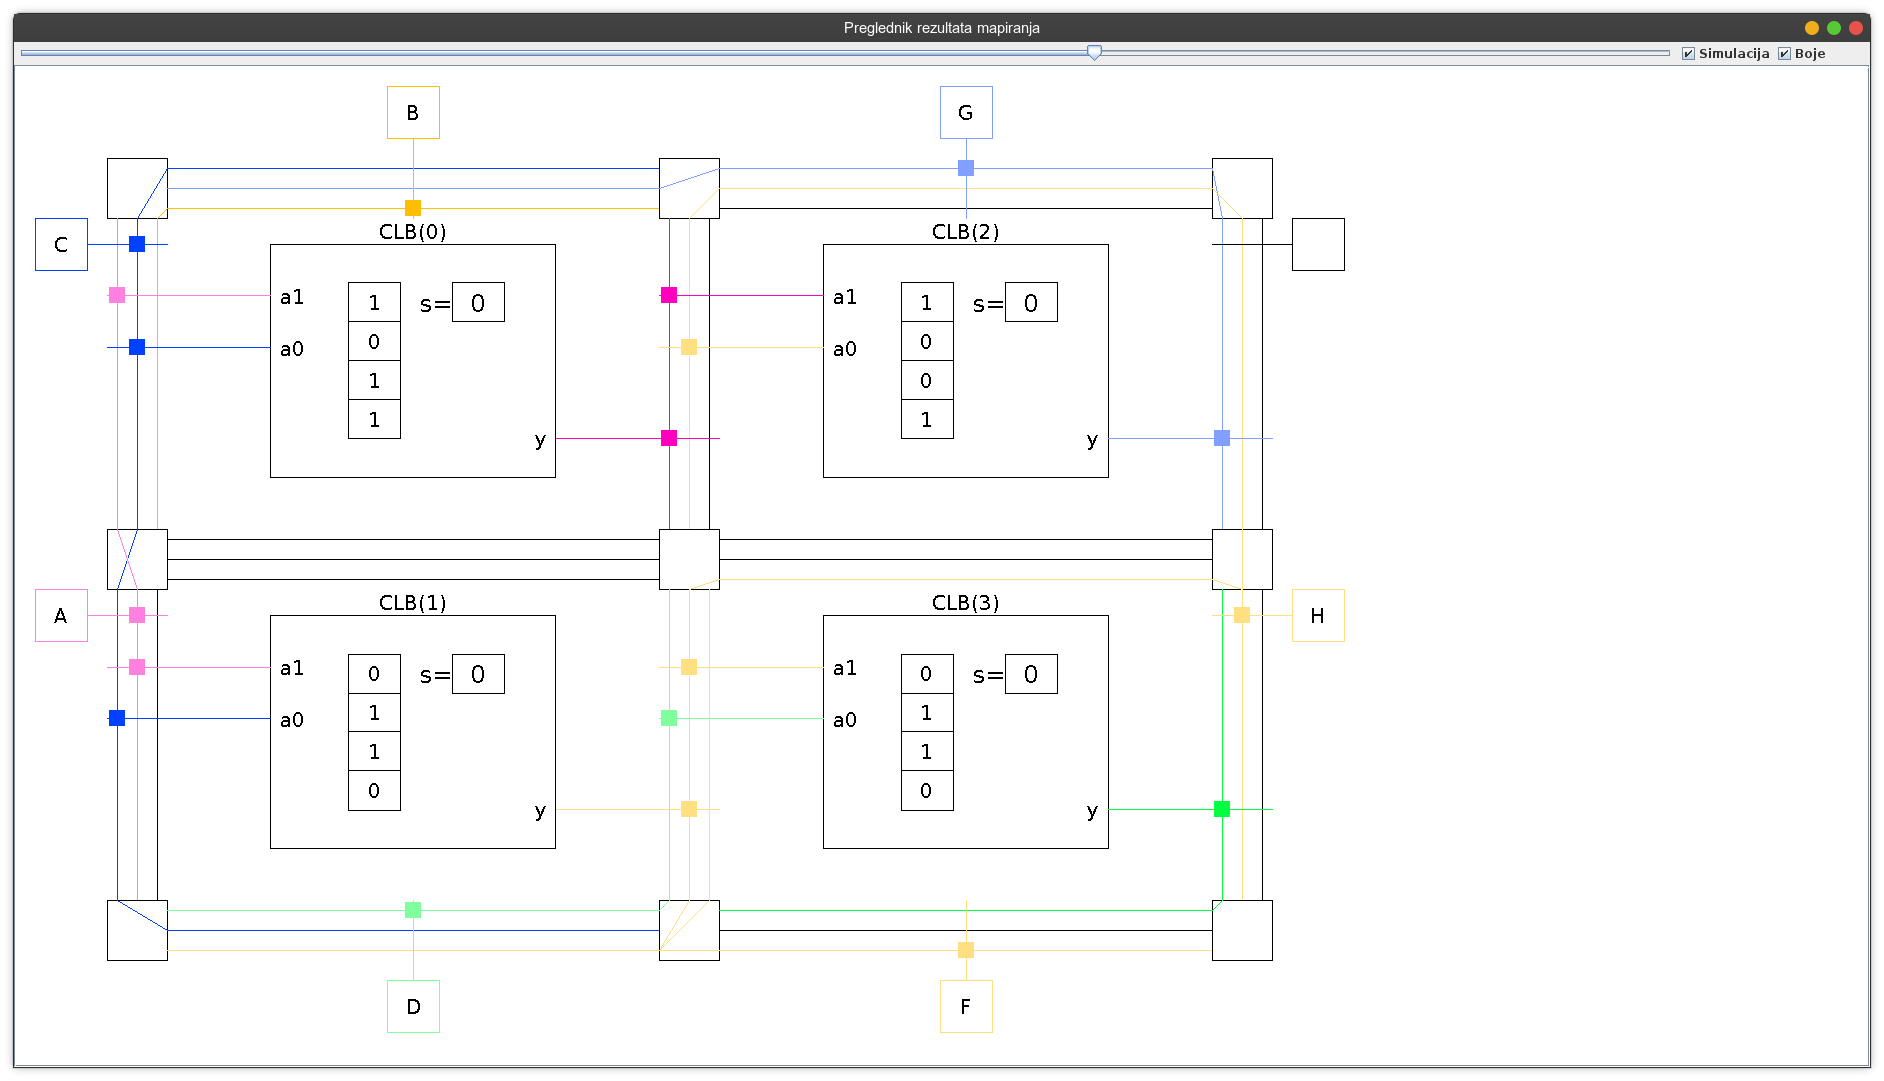
\includegraphics[width=18cm]{slike/conf1.png}
			\caption{Prva moguća "inteligentna" konfiguracija. }
			\label{fig:conf1}
		\end{figure} 
		
		
		\begin{figure}[H]
			\centering
			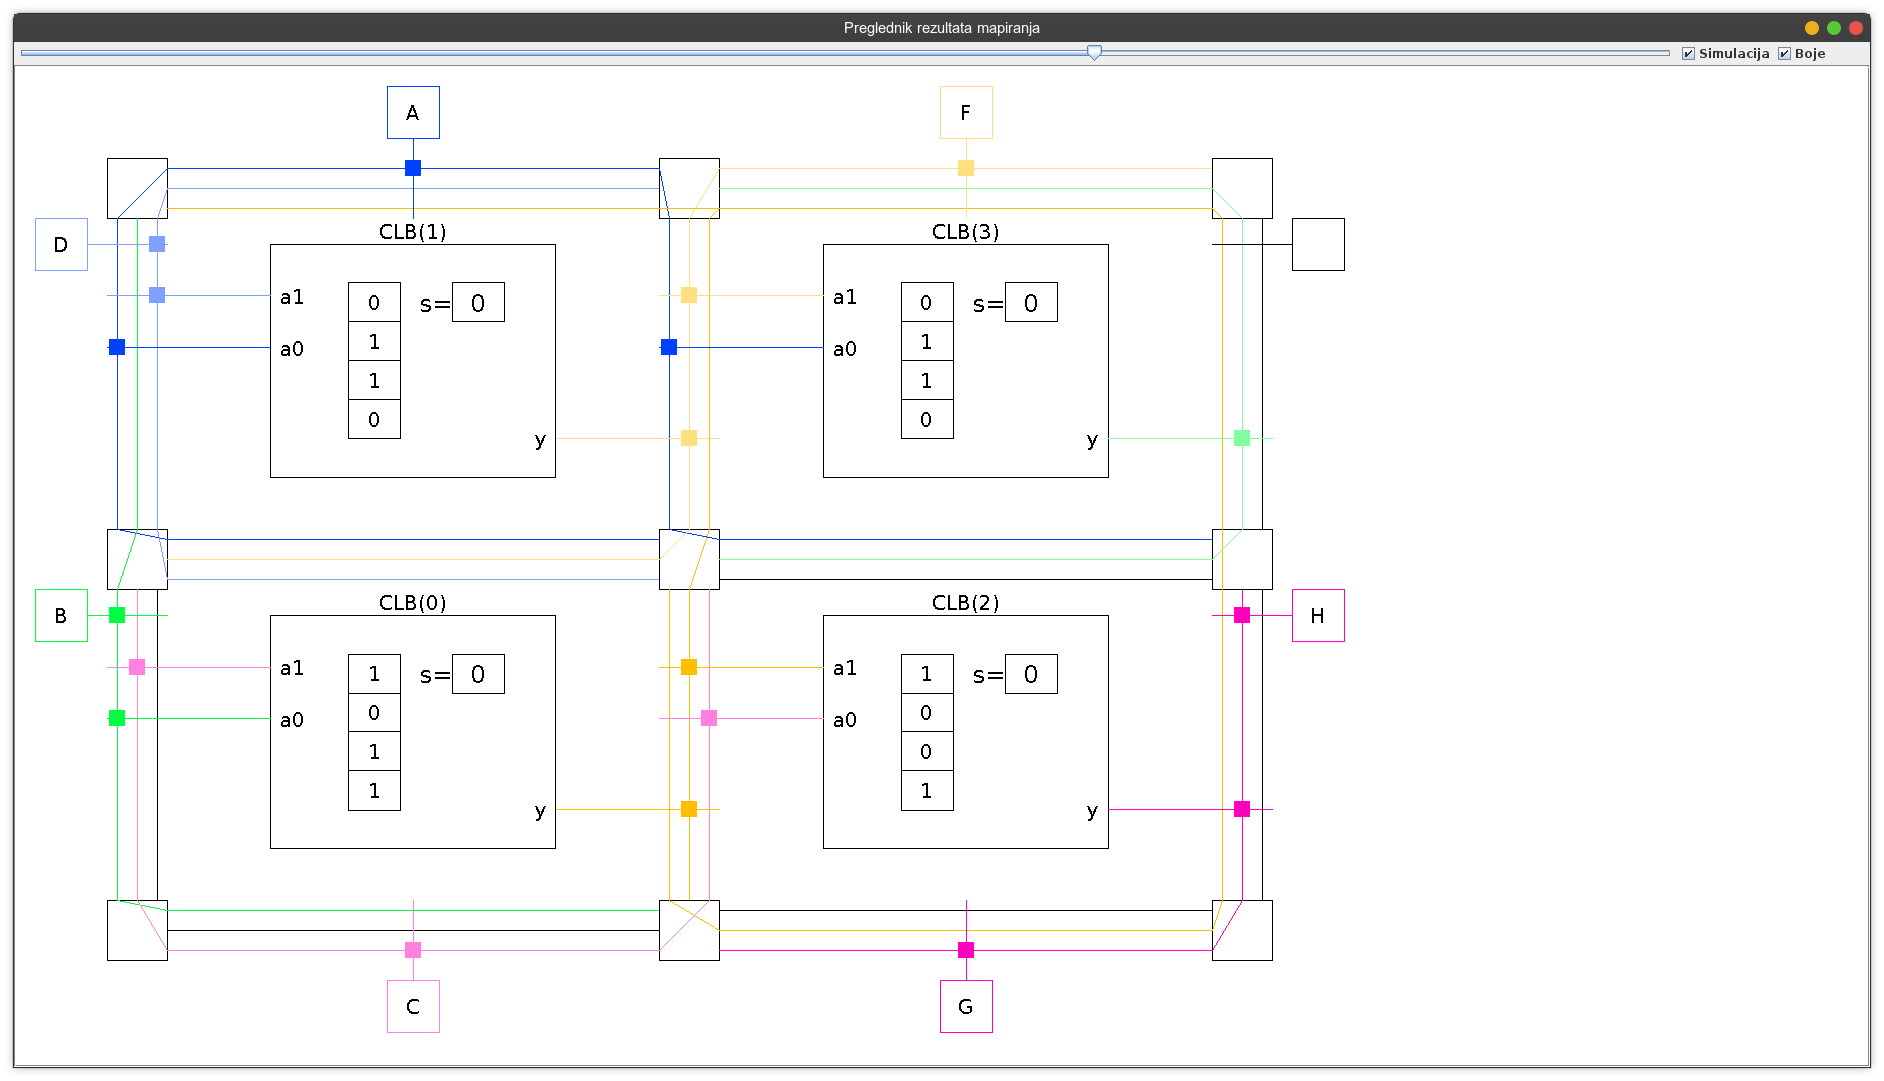
\includegraphics[width=18cm]{slike/conf2.png}
			\caption{Druga "inteligentna" varijanta. }
			\label{fig:conf2}
		\end{figure} 
		
		
		Genetski algoritam je jedan oblik umjetne inteligencije i to je u ovom primjeru jasno potvrđeno. Pri pokretanju algoritma 200 puta, u 49\% slučajeva on je CLB sklopove posložio na jedan od dva gore opisana načina, iako je matematički očekivana vjerojatnost da se to dogodi 2/12 = 16.67\%. 
				
		Složenost problema očituje se i kroz vrijeme potrebno algoritmu da pronađe rješenja. Vrijeme se mjeri u generacijama. Tablice \ref{gen-alg} i \ref{gen-alg-result} pokazuju koliko je u prosjeku potrebno algoritmu da pronađe rješenja za različite slučajeve:
		
		
		\begin{table}[htb]
			\caption{\emph{Rezultati algoritma SV66, s parametrima: Mutacija 5\%, maksimalan broj generacija: 50000, veličina populacije: 50. Broj ponavljanja algoritma: 300}}
			\label{gen-alg-result}
			\centering
			\begin{tabular}{|c | c | c|} \hline
				\thead{Opis} & \thead{Vrijeme u generacijama} & \thead{Uspješnost} \\ \hline
				\makecell{Jedan logički CLB u \\ jedan fizički } & 161.4 & 100\% \\ \hline
				\makecell{Jedan logički CLB u \\ dva fizička, okomito postavljena} & 350.78 & 100\% \\ \hline
				\makecell{Jedan logički CLB u \\ dva fizička, vodoravno postavljena} & 494.23 & 99.9\% \\ \hline
				\makecell{Jedan logički CLB u \\ četiri fizička,2x2 raspored} & 878.2 & 100\% \\ \hline
				\makecell{Dva logička CLB-a s dvije varijable u \\ dva fizička, okomito postavljena} & 5942.72 & 98.33\% \\ \hline
				\makecell{Dva logička CLB-a s dvije varijable u \\ dva fizička, vodoravno postavljena} & 12548.38 & 85.67\% \\ \hline
				\makecell{Dva logička CLB-a s dvije varijable u \\ četiri fizička, 2x2 raspored} & 20422.96 & 70.00\% \\ \hline
				\makecell{Dva logička CLB-a s tri varijable u \\ dva fizička, okomito postavljena} & 14093.15 & 82.33\% \\ \hline
				\makecell{Dva logička CLB-a s tri varijable u \\ dva fizička, vodoravno postavljena} & 18039.90 & 51.67\% \\ \hline
				\makecell{Dva logička CLB-a s tri varijable u \\ četiri fizička, 2x2 raspored} & 30478.80 & 32.33\% \\ \hline
				\makecell{Tri logička CLB-a s tri varijable u \\ četiri fizička, 2x2 raspored} & 31696.92 & 32.67\% \\ \hline
				\makecell{Dva logička CLB-a s tri varijable u \\ četiri fizička, 2x2 raspored, 5 žica} & 21774.24 & 45.00\% \\ \hline
			\end{tabular}
		\end{table}
		
		
		\begin{table}[htb]
			\caption{\emph{Rezultati algoritma SV66, s parametrima: Mutacija 5\%, maksimalan broj generacija: 70000, veličina populacije: 50. Broj ponavljanja algoritma: 300}}
			\label{gen-alg}
			\centering
			\begin{tabular}{|c | c| c|} \hline
				\thead{Opis} & \thead{Vrijeme u generacijama} & \thead{Uspješnost} \\ \hline
				\makecell{Jedan logički CLB u \\ jedan fizički }& 192.21 & 100\% \\ \hline
				\makecell{Jedan logički CLB u \\ dva fizička, okomito postavljena} & 407.56 & 100\% \\ \hline
				\makecell{Jedan logički CLB u \\ dva fizička, vodoravno postavljena} & 455.97 & 100\% \\ \hline
				\makecell{Jedan logički CLB u \\ četiri fizička,2x2 raspored} & 857.57 & 100\% \\ \hline
				\makecell{Dva logička CLB-a s dvije varijable u \\ dva fizička, okomito postavljena} & 6589.83 & 98.67\% \\ \hline
				\makecell{Dva logička CLB-a s dvije varijable u \\ dva fizička, vodoravno postavljena} & 12772.90 & 87.00\% \\ \hline
				\makecell{Dva logička CLB-a s dvije varijable u \\ četiri fizička, 2x2 raspored} & 21226.31 & 78.67\% \\ \hline
				\makecell{Dva logička CLB-a s tri varijable u \\ dva fizička, okomito postavljena} & 16798.01 & 88.33\% \\ \hline
				\makecell{Dva logička CLB-a s tri varijable u \\ dva fizička, vodoravno postavljena} & 21130.95 & 58\%\\ \hline
				\makecell{Dva logička CLB-a s tri varijable u \\ četiri fizička, 2x2 raspored} & 34715.24 & 35\% \\ \hline
				\makecell{Tri logička CLB-a s tri varijable u \\ četiri fizička, 2x2 raspored} & 31322.14 & 38.67\% \\ \hline
				\makecell{Dva logička CLB-a s tri varijable u \\ četiri fizička, 2x2 raspored, 5 žica} & 25162.28 & 50.67\% \\ \hline
			\end{tabular}
		\end{table}
		
		
		\chapter{Zaključak}
		
		U uvodnom dijelu ovog rada dan je teoretski uvod u evolucijsko računarstvo i rad FPGA sklopa. Nakon toga rad se bavi jednom od najvažnijih grana evolucijskog računarstva, a to su genetski algoritmi. Opisano je koje sve vrste genetskog algoritma postoje, što je elitizam, kako utjecati na selekcijski pritisak i kako odabrati i implementirati evolucijske operatore mutacije i križanja. \\
		Implementiran je sustav koji rješava problem smještaja FPGA sklopa, a kroz središnji je dio opisan način izgradnje funkcije dobrote i koji su sve parametri uzeti u obzir pri pronalasku rješenja. Kao selekcijsku metodu korištena je relativna proporcionalna selekcija koja je opisana u poglavlju \ref{proportional-sel}. Križanje i mutacija nisu implementirani nekom od često korištenih jednostavnijih metoda, već je korišten složeniji mehanizam odabira akcije nad dvije odnosno jednom jedinkom. Finalna verzija ovog rada je sustav temeljen na genetskom algoritmu koji provodi mapiranje iz logičkog u fizički svijet, a moguće ga je pokrenuti u trenirajućem načinu rada kroz bash skriptu ./test.sh ili kao jar datoteku koja kao parametar prima konfiguraciju fizičkog CLB-a, put do željene test datoteke, veličinu populacije, broj generacija, broj pokretanja algoritma, ime genetskog algoritma te zastavice koje specificiraju želimo li da se u posebnim dretvama kreiraju grafovi koji opisuju funkciju dobrote i selekcijski intenzitet. Grafovi se spremaju u mape imgs odnosno intensities. Ako se ne pošalju nikakvi parametri, program se pokreće s pretpostavljenim postavkama.Sve greške koje se dogode tijekom izvođenja programa ispisuju se u datoteku exception.txt. \\
		U zadnjem dijelu rada sustav je pokrenut na unaprijed pripremljenim testovima kako bi se odredile klase problema koje genetski algoritam uspješno rješava. Pokazalo se da genetski algoritam za probleme do 3 CLB sklopa uspijeva pronaći rješenja i to u prihvatljivom vremenu < 5s, no veći broj CLB sklopova je prosloženi zadatak za ovaj sustav. Za dodatno poboljšanje potrebno je povećati broj generacija te dodati još parametara u model kako bi genetski algoritam bio ekspresivniji i baratao većim brojem informacija.
		
		
		\bibliography{literatura}
		\bibliographystyle{fer}
		
		\begin{sazetak}
			
			Genetski su algoritmi jedna od metoda evolucijskog računarstva koji imaju široku primjenu. Najčešće se upotrebljavaju za rješavanje kombinatoričkih problema i optimizacijskih problema čija je domena realno područje, no mogu se izuzetno kvalitetno koristiti i za treniranje neuronskih mreža kao alternativa algoritmu propagacije unatrag. Ovaj se rad bavi rješavanjem optimizacijskog problema mapiranja logičkog u fizički FPGA svijet pomoću genetskog algoritma. Pripremljeni su testovi na kojima je izmjerena kvaliteta rada genetskog algoritma. 
			
			\kljucnerijeci{evolucija, metaheuristika, genetski algoritam, optimizacija, kombinatorika, konvergencija, FPGA sklop}
		\end{sazetak}
		
		\engtitle{Solving placement and routing problems in FPGA}
		\begin{abstract}
			
			Genetic algorithms are one of the methods used in evolutionary computing that has many applications. They are used for combinatoric and in optimization problems whose domain is continuum but can also give very satisfying results when used for training neural networks as an alternative to backpropagation algorithm. This paper is dealing with the problem of mapping logical model into physical FPGA model with the help of genetic algorithm. Different tests are prepared for measuring algortihm's quality.
			
			\keywords{evolution, metaheuristics, genetic algorithm, optimisation, combinatorics, convergence, FPGA chip}
		\end{abstract}
		
	\end{document}
	
